\documentclass[11pt,oneside,a4paper]{book}

\usepackage{booktabs}
\usepackage[italian,english]{babel}
\usepackage[utf8]{inputenc}
\usepackage{calligra}
\usepackage[T1]{fontenc}
\usepackage{upquote}
\usepackage{minted}
\usepackage{setspace}
\usepackage{listings}
\usepackage[most]{tcolorbox}
\usepackage{inconsolata}
\onehalfspacing

\newtcblisting[auto counter]{sexylisting}[2][]{sharp corners, 
    fonttitle=\bfseries, colframe=gray, listing only, 
    listing options={basicstyle=\ttfamily,language=java}, 
    title=\thetcbcounter: #2, #1}

\usepackage{amsmath}

\usepackage[top=3cm, bottom=2.5cm, right=2.75cm, left=2.75cm]{geometry}
\usepackage{graphicx}
\usepackage{float}
\usepackage{multicol}
\usepackage{amsmath}

\usepackage{minted}

\setlength{\fboxsep}{0.005pt}
\newcommand{\tmpframe}[1]{\fbox{#1}}
%\renewcommand{\tmpframe}[1]{#1}

\usepackage{float}
\restylefloat{table}


\usepackage{csquotes}

\usepackage{hyperref}
\usepackage[sorting=none]{biblatex}
\addbibresource{bibliografia.bib}

\begin{document}
\selectlanguage{italian}

\title{Sviluppo di un tool per lacomparazione qualitativa di algoritmidi confronto fra stringhe basati sulle Minimal Absent Words}
\author{Antonio Gravino}


\begin{titlepage}
\begin{center}


\includegraphics[width=3cm]{Figure/logo_standard.png}\\
\hfill\\
\begin{spacing}{2.0}
{\LARGE Università degli Studi di Salerno}\\
{\Large Dipartimento di Informatica}\\
\end{spacing}
\hrulefill\\
\vfill
{\Large Corso di Laurea Triennale in Informatica }\\
\vfill\vfill
%{\large Tesi di Laurea in }\\[0.2truecm]
%{\Large Informatica}\\

\begin{spacing}{2.5}
\textbf{\Huge Sviluppo di un tool per la comparazione qualitativa di algoritmi di confronto fra stringhe basati sulle Minimal Absent Words}\\
\end{spacing}
\vfill\vfill

\begin{multicols}{2}
\begin{flushleft}
{\bf Relatrice}\\
Prof.ssa Rosalba Zizza\\
\end{flushleft}
\columnbreak
\begin{flushright}
{\bf Candidato}\\
Antonio Gravino\\
Matricola: 05121 07161\\
\end{flushright}
\end{multicols}

\vfill
\hrulefill 

Anno Accademico 2021/2022

\end{center}
\end{titlepage}

\newpage
\thispagestyle{empty}
\begin{flushright}
\null\vspace{\stretch{1}}
{\calligra{}}
\vspace{\stretch{2}}\null
\end{flushright}


\newpage
\chapter*{}
\thispagestyle{empty}
\hspace*{\fill}\textit{Alla mia famiglia,}

\hspace*{\fill}\textit{faro in un oceano di incertezze.}

\vspace{10mm}

\hspace*{\fill}\textit{Ai miei colleghi universitari,}

\hspace*{\fill}\textit{esempi di vigore e costanza.}

\vspace{10mm}

\hspace*{\fill}\textit{A me,}

\hspace*{\fill}\textit{per aver perseverato nonostante le avversità.}

\vspace{10mm}

\hspace*{\fill}\textit{E infine al popolo ucraino,}

\hspace*{\fill}\textit{che davanti ad un nemico apparentemente invincibile,}

\hspace*{\fill}\textit{ha dato dimostrazione di grande forza e risolutezza,}

\hspace*{\fill}\textit{rinnovando profondamente il mio spirito europeista.}

\vspace{5mm}

\newpage
\thispagestyle{empty}
\begin{flushright}
\null\vspace{\stretch{1}}
{\calligra{}}
\vspace{\stretch{2}}\null
\end{flushright}

\newpage
\tableofcontents
\thispagestyle{empty}

\newpage
\fontsize{13.5}{18.5}\selectfont
\setcounter{page}{1}
\addcontentsline{toc}{chapter}{Abstract}
\chapter*{Abstract}
    \clearpage
\setcounter{page}{1}

{\Huge \textbf{Abstract}}

\vspace{15mm}

Le stringhe sono un potente strumento matematico che si confà ad un spettro ampio e versatile di problematiche, fra cui la bioinformatica. I confronti fra stringhe, fra le altre cose, sono attori centrali nell'evidenziare similiarità delle sequenze genomiche in termine dei loro pattern costituenti.

In letteratura, la maggior parte delle soluzioni algoritmiche al problema dei confronti fra stringhe risultano computazionalmente onerose e prevedono tecniche di confronto allineate; d'altro canto, recenti considerazioni accademiche hanno evidenziato le potenzialità dell'informazione negativa, intesa in questa tesi come \textit{absent words}, nel contesto di confronti alignment-free.

La tesi ha l'obiettivo di integrare un algoritmo alignment-free di confronti fra sequenze che fa uso di \textit{absent words} nel tool String Matching Algorithms Research Tool (SMART), al fine di dimostrare la qualità del risultato.

Forniamo dunque gli elementi matematici fondamentali per la comprensione dell'algoritmo in esame; né elaboriamo, quindi, una codifica prima in pseudocodice e poi in linguaggio di programmazione C; e, infine, procediamo ad integrare il suddetto algoritmo nel tool SMART per ottenere una visione completa della sua resa qualitativa rispetto ad altre soluzioni ben note.
    
\chapter{Introduzione}
    Il confronto fra stringhe è, in generale, un campo di ricerca di largo interesse da parte della comunità scientifica internazionale. Le stringhe risultano una codifica comune per un vasto spettro di oggetti che possono vantare proprietà di confrontabilità. Fra questi, il genoma rappresenta uno dei soggetti  principali dei confronti fra stringhe, essendo banalmente codificabile su un alfabeto ben definito, quale l'alfabeto del genoma. L'analisi del genoma è legata strettamente ai confronti con altre sequenze genomiche, motivo per cui la genomica computazionale ne fa una delle sue principali materie di studio. In generale, la codifica in stringa del genoma permette di individuare caratteristiche qualitative e di rilevare similiarità con filamenti differenti, risultando dunque centrale in ambiti di ricerca internazionali e non.

\vspace{3mm}

In particolare, in questa tesi viene affrontanto il problema degli algoritmi di confronto fra stringhe su alfabeti del genoma con implementazioni \textit{non-allineate} (o \textit{alignment-free}), e cioè che non manipolano la composizione propria della stringa genomica, al fine di ottenere una risultato quanto più efficiente possibile. D'altro canto, il lavoro di tesi riguarda per lo più l'ambito della comparazione qualitativa fra questi algoritmi di confronto fra stringhe; vengono dunque esplorati tool, più o meno recenti, che permettono di effettuare considerazioni di questa natura. Tuttavia, l'assenza di tool significativamente compatibili con gli algoritmi in esame porterà alla realizzazione di un applicativo ad hoc per le necessità evidenziate. 

\vspace{3mm}

Nel Capitolo 2 si introducono nozioni matematiche e cenni teorici fondamentali alla successiva comprensione degli argomenti trattati. Fra le nozioni considerate, le più importanti sono banalmente le \textit{minimal absent words} e la metrica LW, entrambe centrali sia nell'implementazione dell'algoritmo in esame che del tool oggetto di sviluppo; vengono altresì esplorate strutture dati efficienti impiegate in numerose applicazioni nel campo della bioinformatica, come i \textit{suffix arrays}.

Nel Capitolo 3 si analizza con precisione il funzionamento e parte dell'implementazione dell'algoritmo \verb|scMAW|, recente risultato originale di un gruppo di studio che propone una soluzione efficiente circa i confronti fra stringhe impiegando le \textit{minimal absent words}. Si forniscono dettagli sulla costruzione delle strutture matematiche impiegate e sulle modalità di immissione dell'input e restituzione dell'output.

Nel Capitolo 4 si analizza il tool SMART, ideato per ospitare algoritmi di confronto fra stringhe e, in particolare, per individuare il numero di occorrenze di specifici pattern all'interno di testi più o meno voluminosi. Si osserveranno, in particolare, le cause per le quali il tool SMART risulta incompatibile e inoperabile con la specificità degli algoritmi in esame.

Nel Capitolo 5, verrà delineata la realizzazione e lo sviluppo del tool LW Index, che rappresenta il risultato originale di questa tesi di laurea. Verranno fornite specifiche circa i requisiti funzionali dell'applicativo, le scelte progettuali e architettoriali, la selezione delle tecnologie; verrà, inoltre, fornita una panoramica completa sui più importanti componenti dell'implementazione del tool, arricchendo l'esposizione con porzioni di codice ed esempi illustrativi.

Nel Capitolo 6, infine, si effettuano diverse considerazioni sul lavoro svolto e si delineano alcuni possibili sviluppi futuri circa il tool realizzato.

\chapter{Cenni teorici e nozionistici}
    In questa tesi si assumeranno per scontate le nozioni basilari di sequenza, fattore e fattorizzazione, parola, stringa, alfabeto. Inoltre, si assumerà per scontata l'operazione di differenza simmetrica fra due stringhe.

\section{Absent Words, Minimal Absent Words}

Una \textit{absent word} o \textit{parola assente} (detta talvolta \textit{forbidden word} o \textit{parola proibita}) di una certa sequenza $S$ è tale se essa non occorre nella sequenza $S$ stessa. 

Le \textit{absent words} rappresentano, in effetti, la tipologia più genuina di informazione negativa: costituiscono, infatti, un dato che non si presenta in nessuna forma o composizione nella sequenza in esame. In generale, se la sequenza $S$ ha lunghezza $n$, il numero di \textit{absent words} è al più esponenziale in $n$. 

\vspace{3mm}

E' altresì possibile individuare specifiche classi di \textit{absent words}, quali le \textit{minimal absent words}, il cui numero è lineare in $n$. Le \textit{minimal absent words} sono \textit{absent words} di una sequenza $S$ che non occorrono propriamente nella sequenza, ma di cui - invece - tutte le fattorizzazioni proprie occorrono nella sequenza. Si è dunque davanti ad un contrasto interessante: da un lato informazione negativa cruda e grezza; dall'altro, informazione positiva derivata dalla fattorizzazione di informazione negativa. 

\(M_L = \{aub | a,b \in \Sigma*, aub\not\in L, au,ub\in L\} \)

Lo studio di queste fattorizzazioni e la loro applicazione pratica nell'implementazione di \verb|scMAW| ci permetterà di stabilire un metodo efficiente per confrontare stringhe impiegando, alla base, informazione genuinamente negativa.

\vspace{3mm}

Risulta dunque immediato osservare che, impiegando le \textit{minimal absent words} di sequenze $S_1$ e $S_2$, è possibile determinarne la similiarità in tempo proporzionale rispetto alla loro lunghezza $n_1$ e $n_2$, a patto che le due sequenze appartengano al medesimo alfabeto. In particolare, studieremo l'applicazione delle\textit{ minimal absent words} nella cornice dell'alfabeto del genoma $\Sigma_{DNA} =\{A, C, G, T\}$.

\vspace{10mm}

\underline{\textbf{Risultati basati sulle Minimal Absent Words}}

\vspace{5mm}

In letteratura, un moderato numero di risultati sono stati prodotti a partire dalla nozione di \textit{minimal absent words}. Si tratta di soluzioni di complessità, generalmente, $O(n)$, sia in termini di spazio che di tempo, posto e fissato un alfabeto preciso, di lunghezza ben definita. Tuttavia, è interressante osservare la moltitudine di strutture dati impiegate nell'implementazione di questi algoritmi: suffix arrays, suffix trees, suffix automata \cite{CROCHEMORE1998111}, per citarne alcuni. Alcune soluzioni risultano meno performanti di altre, presentando una complessità (nel caso peggiore) pari a $O(n^2 )$ \cite{findingMaw}.

\vspace{3mm}

In questa tesi, presenteremo e analizzeremo - nel Capitolo 3 - l'algoritmo \verb|scMAW|, uno dei più recenti risultati nell'ambito di confronto fra stringhe impiegando le \textit{minimal absent words} e di soddisfacente complessità, sia in termini di tempo che di spazio.

\section{Suffix Arrays}

Come osservato, è possibile introdurre il concetto di minimal absent words impiegando le strutture dati più disparate, come gli automi e i suffix arrays. Questi ultimi sono centrali nell'implementazione dell'algoritmo in esame, quale \verb|scMAW|.

\vspace{3mm}

I suffix arrays, risultato originale del 1990 di Manber-Myers \cite{suffixArray}, sono un array ordinato di tutti i suffissi di una stringa $S$. E' una struttura dati ampiamente utilizzata nell'indicizzazione di testi, negli algoritmi di compressione e nel campo della bibliometrica. La loro complessità è, sia in media che nei casi peggiori, $O(n)$, risultando dunque una struttura dati efficiente e di semplice costruzione.

\vspace{3mm}

In generale, posta $S=S[1]S[2]...S[n]$ una stringa di lunghezza $n$ denotata dai suoi fattori monocarattere, il suffix array $A$ di $S$ è definito come array di interi costituito dalle posizioni iniziali dei suffissi S in ordine lessicografico. $A[i]$ conterrà, in effetti, la posizione iniziale dell'$i$-esimo suffisso più piccolo in $S$. Ogni suffisso compare esattamente una volta. Didatticamente, viene generalmente utilizzata la stringa $banana$ per fornire un esempio.

\vspace{3mm}

Si ponga $S=banana$. Risulta che $S[1]=b, S[2]=a, S[3]=n, ..., S[6]=a, S[7]=blank$. Il $blank$ è generalmente indicato con un trattino basso.

\vspace{3mm}

Si considerino i suffissi di $S$.

\begin{table}[H]
\centering
\begin{tabular}{ll}
\textbf{Suffisso} & \textbf{i} \\
\textit{banana\_} & \textbf{1} \\
\textit{anana\_}  & \textbf{2} \\
\textit{nana\_}   & \textbf{3} \\
\textit{ana\_}    & \textbf{4} \\
\textit{na\_}     & \textbf{5} \\
\textit{a\_}      & \textbf{6} \\
\textit{\_}       & \textbf{7}
\end{tabular}
\end{table}

Ordiniamo i suffissi in ordine lessicografico mantenendo gli indici attuali.

\begin{table}[H]
\centering
\begin{tabular}{ll}
\textbf{Suffisso} & \textbf{i} \\
\textit{\_}       & \textbf{7} \\
\textit{a\_}      & \textbf{6} \\
\textit{ana\_}    & \textbf{4} \\
\textit{anana\_}  & \textbf{2} \\
\textit{banana\_} & \textbf{1} \\
\textit{na\_}     & \textbf{5} \\
\textit{nana\_}   & \textbf{3}
\end{tabular}
\end{table}

Il suffix array $A$ associato conterrà, in maniera associativa, gli indici $i$ soprastanti. Risulterà, dunque, $A[1]=7, A[2]=6, A[3]=4, ..., A[7]=3$.

\vspace{3mm}

E' altrettanto possibile costruire un suffix tree in funzione dei suffix arrays. La costruzione dell'albero è, tuttavia, soggetto alla specificità dell'algoritmo che lo sfrutta.

\section{Range Minimum Queries}

Una range minimum query \cite{RMQ} permettere di trovare il valore minimo in una sottostringa di un array di oggetti confrontabili (nel nostro caso, numeri interi). Sono generalmente utilizzati lateralmente agli LCP (Longest Common Prefix) arrays, quando necessario.

\vspace{3mm}

Dato un array $A[1...n]$ di $n$ oggetti confrontabili e ordinati, il range minimum query $RMQ_A (l,r)$ coincide con $arg_{min} A[k]$, con $1\leq l\leq k \leq r \leq n$. La funzione restituisce la posizione dell'elemento più piccolo nel sotto-array determinato da $A[l...r]$. 

\vspace{3mm}

Ad esempio, per l'array $A=0,5,2,5,4,3,1,6,3$, risulterà che il range minimum query di $A[3...8]=2,5,4,3,1,6$ è 7, poiché $A[7]=1$ ne é il valore più piccolo, dunque il minimo, ottenuto tramite confronti più o meno lineari.

\vspace{3mm}

La nozione di range minimum queries è, analogamente a quella di suffix arrays, centrale alla costruzione dell'algoritmo \verb|scMAW|.

\section{Metrica LW di Crochemore}

Chairungsee e Crochemore del King's College di Londra hanno presentato, nel 2012, una misura di similiarità fra due stringhe $x$ e $y$ impiegando le \textit{minimal absent words} \cite{CHAIRUNGSEE2012109} di ciascuna delle due, rispettivamente $M^l_x$ e $M^l_y$, dove $l$ è la lunghezza massima fra le due stringhe.

\vspace{3mm}

\textit{LW Index} sta per \textit{Length-Weighted Index}.

\vspace{3mm}

La metrica, che restituisce un float, è calcolata come sommatoria di $\frac{1}{|w|^2}$ dove ogni $w$ è una parola ottenuta dalla differenza simmetrica fra le minima absent words di $x$ e di $y$.

\[LW_l (x, y)=\sum_{w \in M^l_x \Delta M^l_y} \frac{1}{|w|^2 }\]

\vspace{3mm}

Ricordiamo, inoltre, che la \textit{differenza simmetrica} fra due insiemi $X$ e $Y$ è definita come unione fra la differenza tra il primo insieme e il secondo insieme, e la differenza fra il secondo insieme e il primo insieme. Si osservi che il motivo per cui la metrica fa uso dell'inverso delle stringhe è proprio a causa della differenza simmetrica stessa.

\vspace{3mm}

In generale, nell'implementare l'algoritmo \verb|scMAW| considereremo una più generica metrica LW che non tiene conto della lunghezza $l$.

\[LW (x, y)=\sum_{w \in M_x \Delta M_y} \frac{1}{|w|^2 }\]

Ad esempio, posto $x=abaab$ e $y=aabbbaa$, risulterà che $M_x=aaa, aaba, bab, bb$ (osserviamo che tutte le fattorizzazioni di $M_x$ sono presenti in $x$) e $M_y=aaa,bbbb,aba,abba,bab,baab$.

\vspace{3mm}

Risulterà:

\vspace{3mm}

\(M_x \Delta M_y ={aaba,aba,abba,baab,bb,bbbb}\)

\vspace{3mm}

Di consequenza, il soprastante risultato verrà dato in pasto alla sommatoria produttrice della metrica LW. Ogni lunghezza (inversa, ed elevata al quadrato) degli elementi dell'insieme ($aaba$, $aba$, ...) sarà sommata, al fine di produrre la metrica.

\(LW(x,y) = \frac{1}{4^2}+\frac{1}{3^2}+\frac{1}{4^2}+\frac{1}{4^2}+\frac{1}{2^2}+\frac{1}{4^2}\)

Questa misura permette di quantificare la distanza fra due parole, definendone la similitudine. Risulta, infatti, $LW(x,x)=0$. 

\chapter{Analisi dell'algoritmo scMAW}
    Nel 2018, un gruppo di studio internazionale composto da studenti del King's College di Londra, dell'Università di Palermo e dell'Universitità di Loughborough (Regno Unito), ha proposto una soluzione efficiente ed originale in merito al problema del confronto fra stringhe impiegando le minimal absent words, la cui nozione è descritta nel Capitolo 2. 

\vspace{3mm}

Al tempo della stesura del paper relativo all'algoritmo in questione \cite{scMAW}, gli algoritmi dalla complessità migliore, generalmente $O(n)$ in media e $O(n^2 )$ nei casi peggiori, impiegavano strutture dati variegate, alcune più o meno adatte a trattare l'informazione negativa rappresentata dalle minimal absent words. 

\vspace{3mm}

Analogamente, il gruppo di studio decise di sfruttare una metrica originale, precedentemente introdotta da Chairungsee e Crochemore \cite{CHAIRUNGSEE2012109}, chiamata Metrica LW, o Indice LW. 

\vspace{3mm}

L'indice permette di definire la similiarità, o similitudine, fra due stringhe - generalmente su un alfabeto ben definito, come quello genomico o proteico - in funzione delle loro minimal absent words, ed in particolare sulla loro differenza simmetrica, generalmente calcolabile con complessità $O(m+n)$ in media, con $m$ e $n$ le lunghezze delle stringhe in input.

\vspace{3mm}

La prima sfida posta dall'algoritmo giaceva nella ricerca delle loro minimal absent words. Il gruppo di studio ha deciso di utilizzare soluzioni ben note, delineate in \cite{maw1}. 

Questo risultato accademico dimostra che è possibile computare, poste due stringhe $x$ e $y$, le corrispettive minimal absent words $M_x$ e $M_y$ in tempo lineare relativo alle lunghezze delle stringhe, rispettivamente $n$ e $m$. 

\vspace{3mm}

La strategia fondamentale dell'algoritmo, d'ora in poi denominato in questo Capitolo come \verb|scMAW|, è di effettaure una \textit{merge-sort} dei due insiemi $M_x$ e $M_y$, unendoli dopo che i due insiemi sono stati ordinati tramite l'ausilio dei suffix arrays. 

\vspace{3mm}

A questo fine, verrà costruito il suffix array associato alla parola $w=xy$. Questa struttura può essere costruita con complessità di tempo e spazio $O(m+n)$. Attraverso questa struttura dati, è immediato ordinare in maniera lessicografica (e cioè tramite i suffissi delle parole associate) i due insiemi di minimal absent words. 
Questo significa che gli insiemi sono considerati associati se, posti $x_1$ e $x_2$ tuple di uno degli insiemi, $x_1 < x_2$ se la prima lettera dopo il \textit{longest common prefix} di $x_1$ è lessicograficamente più piccola di quella di $x_2$. 

In generale, il \textit{longest common prefix} è una struttura prodotta a partire dal preprocessamento di un suffix array. E' intuitivo individuarne la relazione: i suffix array lavorano ai suffissi, che in maniera laterale possono condurre al calcolo dei prefissi.

\section{Computazione dell'insieme \(M_{x,y}\) e di \(LW(x,y)\)}

Una volta ordinati $M_x$ e $M_y$, è possibile procedere con la merge. Si tratta di un'operazione elementare. L'obiettivo è costruire l'insieme $M_{x,y} = M_x U M_y$ utilizzando due indici incrementali $i$ e $j$, tali che l'insieme non contenga ridondanze e sia, al termine della computazione, ordinato. L'insieme è dunque definito come segue.

\begin{equation*}
  \left\{
    \begin{aligned}
      & {\left|
        M_{x,y} U \{x_i \}
      \right|} \text{ e incrementa } i\text{, se } x_i < y_j \\
      & {\left|
        M_{x,y} U \{y_j \}
      \right|} \text{ e incrementa } j\text{, se } x_i > y_j \\
      & {\left|
        M_{x,y} U \{x_i = y_j \}
      \right|} \text{ e incrementa } i,j\text{, se } x_i = y_j \\
    \end{aligned}
  \right.
\end{equation*}

Contemporaneamente alla costruzione dell'insieme $M_{x,y}$ è possibile costruire l'indice delle similitudini fra le stringhe calcolando $LW(x,y)$ e seguendo l'incremento degli indici $i$ e $j$. La costruzione di tale valore è l'obiettivo finale dell'algoritmo, nonché l'output della sua implementazione. E' banale osservare che il calcolo produrrà un \textit{float}.

\begin{equation*}
  \left\{
    \begin{aligned}
      & {\left|
        LW(x,y) + \frac{1}{|x_j |^2}
      \right|} \text{ e incrementa } i\text{, se } x_i < y_j \\
      & {\left|
        LW(x,y) + \frac{1}{|x_j |^2}
      \right|} \text{ e incrementa } j\text{, se } x_i > y_j \\
      & {\left|
        LW(x,y)
      \right|} \text{ e incrementa } i,j\text{, se } x_i = y_j \\
    \end{aligned}
  \right.
\end{equation*}

E' interessante osservare che quando $x_i = x_y$, l'indice $LW(x,y)$ non incrementa. In alternativa, quando $x_i =/= x_y$, l'indice incrementa in funzione della composizione propria della parola, delineata in base al quadrato della sua cardinalità.

\vspace{3mm}

I calcoli elementari nell'algoritmo, come le somme, hanno complessità costante; vengono, altresì, effettuate per ogni tupla in $M_x$ e $M_y$: è dunque possibile concludere che l'intera operazione richieda $O(m+n)$

\vspace{3mm}

E' importante sottolineare che questo algoritmo è disponibile in una controparte dedicata alle sequenze circolari; tuttavia, questa tesi si limiterà ad analizzare unicamente il risultato ottenuto per le sequenze lineari.

\section{Implementazione e versioning}

Le implementazioni di \verb|scMAW| utilizzano, per la ricerca delle minimal absent words e il conseguente popolamento degli insiemi $M_x$ e $M_y$, algoritmi già noti, a cui ci si riferirà come $MAW$. \verb|scMAW| è stato implementato nel linguaggio C. 

Ammette, come input, un file in formato FASTA (o MultiFASTA) con una formattazione ben precisa, definita nel Capitolo 5, ed un parametro che indica se valutare le sequenze in input come lineari o circolari. 

Restituisce, come output, un file (generalmente FASTA.OUT, oppure PHYLIP) formattato come altresì descritto nel Capitolo 5. 

\vspace{3mm}

In generale, il suddetto file d'output presenterà una matrice, dove ogni cella $[x,y]$ denoterà il corrispettivo indice $LW(x,y)$. Il file risulta di lettura più o meno immediata, consentendone dunque il processamento da parte di un software come il tool LW Index, la cui realizzazione originale è ampiamente descritta nel Capitolo 6.

\vspace{3mm}

Il codice sorgente di \verb|scMAW| è disponibile su GitHub \cite{mawGit}.

\vspace{3mm}

La root della repository contiene, per lo più, file di installazione e compilazione (Makefile, pre-install.sh, INSTALL), informativi e/o di copyright (LICENSE, README), e collezioni di strutture dati e funzioni generiche impiegate negli algoritmi, fra cui \verb|MAW| (stack, maw). La root contiene anche diverse subdirectory, fra cui una cartella denominata \verb|scMAW|, che contiene l'implementazione dell'omonimo algoritmo in esame.

\vspace{3mm}

La directory contiene due subfolders, \verb|data| ed \verb|exp|. Il primo contiene alcuni file FASTA di esempio, popolate con stringhe casuali sull'alfabeto del genoma. La seconda, invece, contiene i corrispettivi file di output generati a partire dai file in input nella prima cartella. 

La cartella è popolata con numerosi file, per lo più di installazione.  Gli unici file relativi al risultato originale sono \verb|functions| e \verb|mawdefs|. Il secondo file è fondamentalmente uno snapshot a basso livello delle funzioni impiegate, successivamente, nel primo file. 

Si tratta di funzioni come \verb|getMaws(..)| (per computare e popolare gli insiemi $M_x$ e $M_y$) e \verb|maw_seq_comp(..)| per l'effettivo computo degli indici $LW(x,y)$. La maggior parte delle funzioni sono per lo più ausiliari e di scarso interesse. Le altre funzioni presenti, come la creazione del file di output e la stampa dei risultati, hanno generalmente lo scopo di coadiuvare il computo (es. predisporre le strutture dati necessarie) e/o occuparsi del pre-computo o post-computo (es. leggere il file di input o generare il file di output).

\vspace{3mm}

La codifica degli algoritmi è il corrispettivo in C si assesta sull'ordine delle migliaia di righe e non risulta di conseguenza opportuno includerne porzioni decontestualizzate in questo documento; si invita, dunque, a consultare, in caso di interesse, la repository che ne deposita il codice sorgente.

\chapter{Analisi del tool SMART}
    Lo String Matching Algorithm Research Tool, da qui in poi SMART \cite{smart}, è un tool dedicato ai ricercatori e a gli studenti di algoritmi di confronto fra stringhe. Il tool offre un ambiente versatile, scalabile e facilmente integrabile con nuovi algoritmi per effettuare considerazioni qualitative nella cornice dei problemi derivati dalla più ampia materia del \textit{pattern matching}. In generale, SMART propone un framework di lavoro adatto a testare, progettare, valutare e comprendere le soluzioni del problema del confronto fra stringhe. 

\vspace{3mm}

Il tool è stato sviluppato da un gruppo accademico internazionale \cite{smartHomepage}, il quale ha successivamente rilasciato il codice sorgente dell'applicativo su GitHub in una repository pubblica. Il tool ha successivamente ricevuto una moderata documentazione ai fini di coadiuvare i futuri sviluppatori che intendessero estendere le funzionalità del tool o, più banalmente, integrare nuovi algoritmi di confronto fra stringhe \cite{smartHelp}.

\vspace{3mm}

E' possibile utilizzare SMART in ambiente Windows, MAC OS X e Linux. Per semplicità, si è deciso di utilizzare una macchina virtualizzata montata con Ubuntu 64bit. L'ambiente di lavoro barebones e Unix-based ha permesso al tool di lavorare al massimo dell'efficienza e senza alcun disguido di natura tecnica, che avrebbero potuto aver luogo in contesti non-Unix, come Windows e MAC OS X, soprattutto in termini di compatibilità con librerie e dipendenze di cui SMART fa ampiamente uso.

\section{Funzionamento di SMART}

\begin{figure}[ht!]
    \centering
    \tmpframe{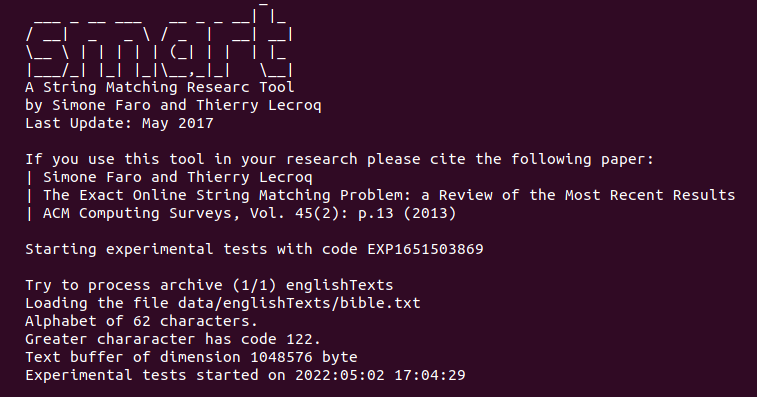
\includegraphics[width=6in]{Figure/smartWelcome.png}}
    \caption{Schermata di benvenuto del tool SMART.}
    \label{fig:esempio}
\end{figure}

Ad alto livello, il tool SMART:

\begin{itemize}
    \item Permette di selezionare al più $N$ algoritmi $A+$, dove:
    \begin{itemize}
        \item $A+$ è un algoritmo che sia testato, funzionante e \textit{valido}. Un algoritmo $A$ non testato, funzionante o valido non può essere selezionato. Una volta testato tramite gli appropriati strumenti offerti dal tool, un simbolo $+$ viene utilizzato per indicare la traslazione di stato da algoritmo non selezionabile $A$ ad algoritmo selezionabile $A+$.
        \item $N$ è il numero di algoritmi disponibili. In particolare, $N$ non coincide necessariamente con i sorgenti degli algoritmi presenti nel filesystem del tool, bensì con il numero di algoritmi presenti nella cartella \verb|~root/sources/algos| al momento della compilazione e del bundling tramite \verb|Makefile|. Il processo è descritto nel dettaglio in seguito.
    \end{itemize}
    \item Permette di selezionare uno o più testi $T$ su cui lanciare la computazione. I testi, incapsulati in file TXT, sono fra i più variegati:
    \begin{itemize}
        \item Testi accademici o letterari scritti in linguaggio naturale e in lingue diverse. Di default, SMART offre testi in lingua italiana, inglese, francese e cinese. Si tratta di testi narrativi più o meno lunghi, oppure di articoli accademici di dominio pubblico. La lunghezza di questi testi si aggira sulle centinaia di migliaia di parole.
        \item Descrizioni del genoma. Insiemi di stringhe su alfabeti DNA o PROT. 
    \end{itemize}
    \item Permette di selezionare l'upper bound e il lower bound dei pattern da riscontrare nelle sequenze. In generale, SMART confronta le stringhe in input in funzione dei loro pattern costituenti: è possibile, dunque, specificare una lunghezza minima e massima dei suddetti pattern; all'esecuzione, il tool incrementerà la lunghezza dei pattern in maniera esponenziale (ad esempio, potrebbe iniziare confrontando le stringhe con pattern di lunghezza 2, poi 4, 8, 16, 32 e così via). E' anche possibile determinare specifiche regioni di testo sulla quale ricercare i pattern.
    \item Una volta selezionato almeno $1$ algoritmo $A+$ e almeno un testo $T$, ed eventualmente aver definito parametri limitativi sui pattern da rilevare nelle stringhe accolte, è possibile lanciare l'applicativo. Il terminale verrà popolato da barre di caricamento sufficientemente descrittive che segnaleranno l'avanzamento della computazione. Una volta conclusa, SMART indicizzerà l'esperimento con l'attuale $timestamp$ seguendo una nomenclatura precisa (es. $EXP20220203$). 
    
    \begin{figure}[ht!]
    \centering
    \tmpframe{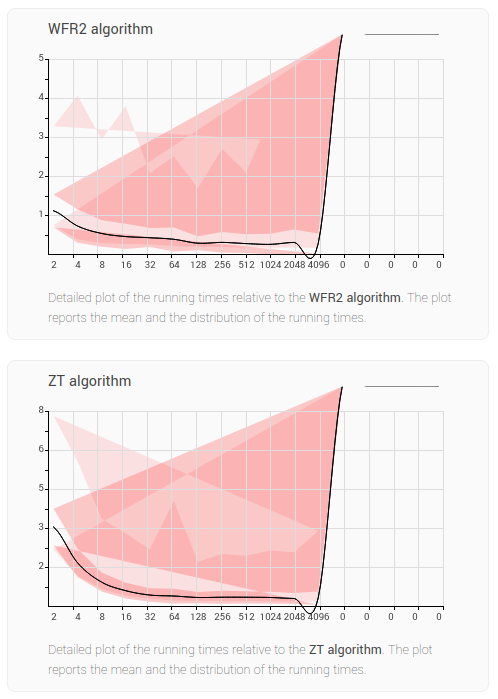
\includegraphics[width=5in]{Figure/smartDistribution.png}}
    \caption{Dettaglio di un grafico sulla \textit{Distribution} generato da SMART relativo a due algoritmi: WFR2 e ZT.}
    \label{fig:esempio}
\end{figure}
    
    Il tool creerà una cartella in \verb|/results| col nome dell'esperimento e inserirà in quest'ultima i risultati ottenuti sotto forma di alcune pagine HTML elaborate con CSS e JavaScript. La pagina conterrà, essenzialmente, dei grafici informativi sulla computazione appena effettuata, dando spazio a considerazioni di natura qualitativa e comparativa degli algoritmi $A+$ selezionati in funzione dei testi $T$ impiegati.
\end{itemize}

\begin{figure}[ht!]
    \centering
    \tmpframe{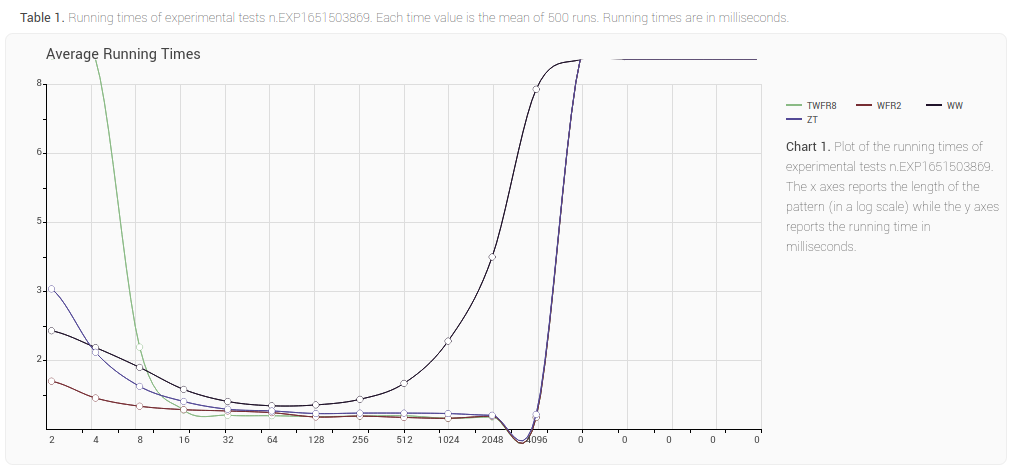
\includegraphics[width=6in]{Figure/smartGraph.png}}
    \caption{Dettaglio di un grafico sull'\textit{Average Running Time} generato da SMART.}
    \label{fig:esempio}
\end{figure}

\subsection{Installazione e compilazione}

Analizzando il codice sorgente di SMART su GitHub \cite{smartGithub} è possibile delineare il funzionamento sia ad alto livello che a basso livello del tool. In generale, gli sviluppatori hanno previsto un processo di installazione immediato: è sufficiente infatti clonare la repository tramite GitHub ed avviare il processo di compilazione e bundling tramite \verb|Makefile|: 

\begin{verbatim}
https://github.com/smart-tool/smart.git
cd smart-tool
./makefile
\end{verbatim}

E' importante osservare che è necessario ricompilare tramite \verb|Makefile| ogni qual volta s'intende integrare un nuovo algoritmo. Infatti, il processo di bundling è esteso alle sotto-directory della \verb|~root|, inclusa la folder \verb|/bin|, che conterrà i file binari di output degli algoritmi. In generale, il filesystem di SMART è così strutturato:

\subsection{Struttura del filesystem}

\begin{itemize}
    \item \verb|~root|: Contiene una serie di eseguibili extension-less lanciabili tramite terminale, fra cui \verb|./SMART| e \verb|./SELECT|. Un ulteriore eseguibile è disponibile per verificare la correttezza dei nuovi algoritmi da integrare nel tool.
    \begin{itemize}
        \item \verb|./SMART|: E' il core dell'applicativo. Da linea di comando, ammette un insieme di opzioni che permettono di descrivere l'input del programma, l'alfabeto utilizzato, la lunghezza massima dei pattern da ricercare nelle stringhe, nonché ulteriori flag opzionali per confronti più specializzati.
        \item \verb|./SELECT|: analogamente all'eseguibile SMART, ammette una serie di opzioni che hanno l'obiettivo di determinare gli algoritmi da utilizzare quando si lancerà il prossimo confronto con SMART. I comandi ammessi, fra gli altri, sono \verb|-show| (stampa un elenco esaustivo degli algoritmi selezionabili), \verb|-none| (deseleziona tutti gli algoritmi), \verb|-all| (seleziona tutti gli algoritmi) e \verb|[ALGO_NAME]| (seleziona uno specifico algoritmo, a patto che sia presente nella cartella \verb|/algos|. Il comando \verb|-which| permette di identificare gli algoritmi attualmente selezionati e in procinto di essere computati con la prossima invocazione del comando \verb|./SMART|. Infine, il comando \verb|-add| permette di integrare nuovi algoritmi nel tool: è un comando centrale nel funzionamento ad alto livello di SMART, poiché permette a sviluppatori esterni di estenderne le prospettive computative.
        
        \begin{figure}[ht!]
        \centering
        \tmpframe{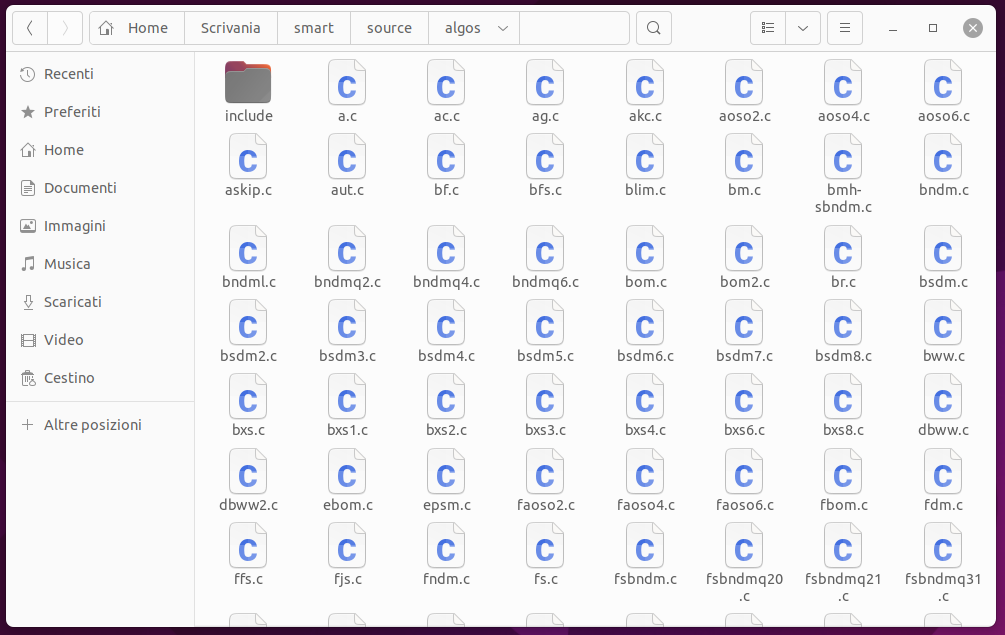
\includegraphics[width=5.5in]{Figure/smartAlgos.png}}
        \caption{Contenuto della cartella ALGOS. L'anteprima non mostra la presenza di una sottocartella BIN, motivo per cui è immediato assumere che l'attuale istanza di SMART non sia stata ancora compilata tramite MAKEFILE.}
        \label{fig:esempio}
        \end{figure}
    \end{itemize}
    La root del filesystem contiene anche file di copyright e guide all'installazione del software.
    \item \verb|/data|: contiene una serie di sottocartelle descrittive dei possibili testi da fornire in input al programma. Ad esempio, la cartella \verb|/data/englishTexts| contiene \verb|bible.text| e \verb|index.txt|. Il primo conterrà il testo grezzo in UTF-8; il secondo conterrà alcune informazioni di indicizzazione del testo per permettere all'applicativo di utilizzarlo come input. Di default, infatti, il testo in inglese di riferimento è la trascrizione della Bibbia; invece, i testi in italiano di riferimento sono, fra gli altri, l'Orlando furioso, la Divina Commedia e le Ultime lettere di Jacopo Ortis. Il file \verb|data/italianTexts/index.txt| sarà così strutturato:
    
    \begin{sexylisting}{data/italianTexts/index.txt}
La divina commedia
Dante Aligheri (1307)
[url della fonte]
#la_divin.txt#
551,9 kB

Orlando furioso
Ludovico Ariosto (1532)
[url della fonte]
#orlando_.txt#
1,5 MB

Ultime lettere di Jacopo Ortis
Ugo Foscolo (1817)
[url della fonte]
#ultime_l.txt#
281,2 kB

    \end{sexylisting}
    \item \verb|/results|: contiene tante sottocartelle quanti gli esperimenti (eg. \textit{computazioni}) elaborati tramite SMART. I nomi delle cartelle seguono una nomenclatura univoca, come descritto in precedenza, e associano ad ogni esperimento un preciso identificativo, determinato dal timestamp.
    \item \verb|/source|: contiene i file sorgenti C del core del software (ad esempio \verb|./smart.c| per l'eseguibile \verb|./SMART/|) e degli algoritmi di confronto fra stringhe disponibile. Circa 80 algoritmi sono disponibili di default, e nuovi sono integrabili. In particolare:
    \begin{itemize}
        \item La cartella \verb|/algos| contiene i file sorgenti C degli algoritmi, strutturati in modo specifico al fine di poter essere compatibili col tool. Il \verb|Makefile| di SMART compilerà questi file sorgente C in binari di output. 
        \item La cartella \verb|/bin| contiene i file binari risultato della compilazione dei sorgenti in C di \verb|/algos|. In effetti, questi file binari sono esattamente quelli utilizzati durante i processi computazionali del tool. 
    \end{itemize}
\end{itemize}

\section{Integrazione di nuovi algoritmi}

Per aggiungere un nuovo algoritmo al tool SMART, è necessario creare un file sorgente in C nella cartella \verb|~root/source/algos| e notificare il tool della sua presenza tramite \verb|./select -add [ALGO_NAME]| dopo averlo opportunamente testato e validato tramite le strumentazioni automatiche del tool. 

\vspace{3mm}

Il contenuto del file C dev'essere compatibile con il modo di computare i confronti fra stringhe e le ricerche di pattern di SMART. L'algoritmo può utilizzare $include$ esterni, come librerie e altre forme di dipendenze programmatiche. Il file sorgente può includere una serie di funzioni ausiliare per favorire il riuso e la leggibilità, oppure per motivi di iterazione o ricorsione. Tuttavia, SMART prevede che almeno una funzione (definita come tale) sia presente nel sorgente C, e che questa funzione abbia una firma ben definita.

\begin{figure}[ht!]
    \centering
    \tmpframe{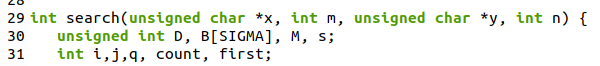
\includegraphics[width=5.5in]{Figure/smartAlgoSign.png}}
    \caption{Firma di un algoritmo predefinito di SMART. Il contenuto della funzione è irrilevante, ma la firma è cruciale.}
    \label{fig:esempio}
\end{figure}

In particolare, la funzione in questione, denominata $search$, deve restituire un intero e accogliere esattamente tre parametri nel seguente ordine:
\begin{itemize}
    \item \verb|unsigned char *x|, pattern da ricercare all'interno del testo $*y$
    \item \verb|int *m|, lunghezza del pattern \verb|*x|
    \item \verb|unsigned char *y|, testo sul quale ricercare il pattern \verb|*x|
    \item \verb|int *n|, lunghezza del testo \verb|*n|
\end{itemize}

Se l'algoritmo non trova alcuna occorrenza del pattern, l'algoritmo dovrà restituire $-1$. In alternativa, dovrà \textbf{restituire \textit{esattamente} il numero di occorrenze del pattern} $*x$ nel testo $*y$.

Il contenuto della funzione è irrilevante, a patto che rispetti i requisiti soprastanti. Questo significa che è possibile usare qualsiasi struttura dati, tecnica algoritmica e metodo di computazione per arrivare all'intero richiesto. La complessità dell'algoritmo è altresì irrilevante e non vincolante all'implementazione o all'integrazione con SMART; sarà difatti compito del tool effettuare le dovete comparazioni degli algoritmi.

\begin{figure}[ht!]
    \centering
    \tmpframe{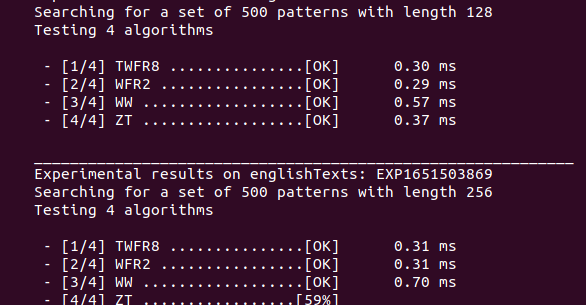
\includegraphics[width=5.5in]{Figure/smartComputing.png}}
    \caption{Porzione di una fase del processo di computazione di SMART. In questa anteprima, SMART sta computando quattro algoritmi: TWFR8, WFR2, WW e ZT. In particolare, sta ricercando un preciso numero di pattern (500) di lunghezza esponenziale (128, 256). Ogni riga presenta il tempo richiesto in millisecondi.}
    \label{fig:esempio}
\end{figure}

E' possibile validare l'algoritmo attraverso il comando \verb|./TEST [ALGO_NAME]|. Il tool tenterà di e, se il numero di occorrenze restituito dall'algoritmo testato coinciderà con l'intero che il tool si aspetta, allora l'algoritmo sarà considerato valido, testato e pienamente funzionante; sarà possibile, a questo punto, integrarlo e selezionarlo tramite \verb|./SELECT|.


\section{Accenni al versioning parallelo di SMART-GUI}

Gli autori del tool SMART, per venire incontro a prerogative di usabilità, hanno deciso di sviluppare una versione parallela che, invece di poter essere utilizzata esclusivamente da linea di comando, sia invece adoperabile tramite un'interfaccia grafica. Questa versione è stata denominata SMART-GUI ed è disponibile su GitHub \cite{smartGUI}. 

\vspace{3mm}

Il funzionamento è del tutto analogo alla sua controparte da terminale. L'unica sostanziale differenza è, appunto, l'introduzione di un'interfaccia grafica, che sostituisce i comandi principali dell'applicativo da CLI, come \verb|./SMART| e \verb|./SMART|, adesso integrati in un'unica finestra sotto forma di riquadri di input, tabs e bottoni interattivi.

\vspace{3mm}

\begin{figure}[ht!]
    \centering
    \tmpframe{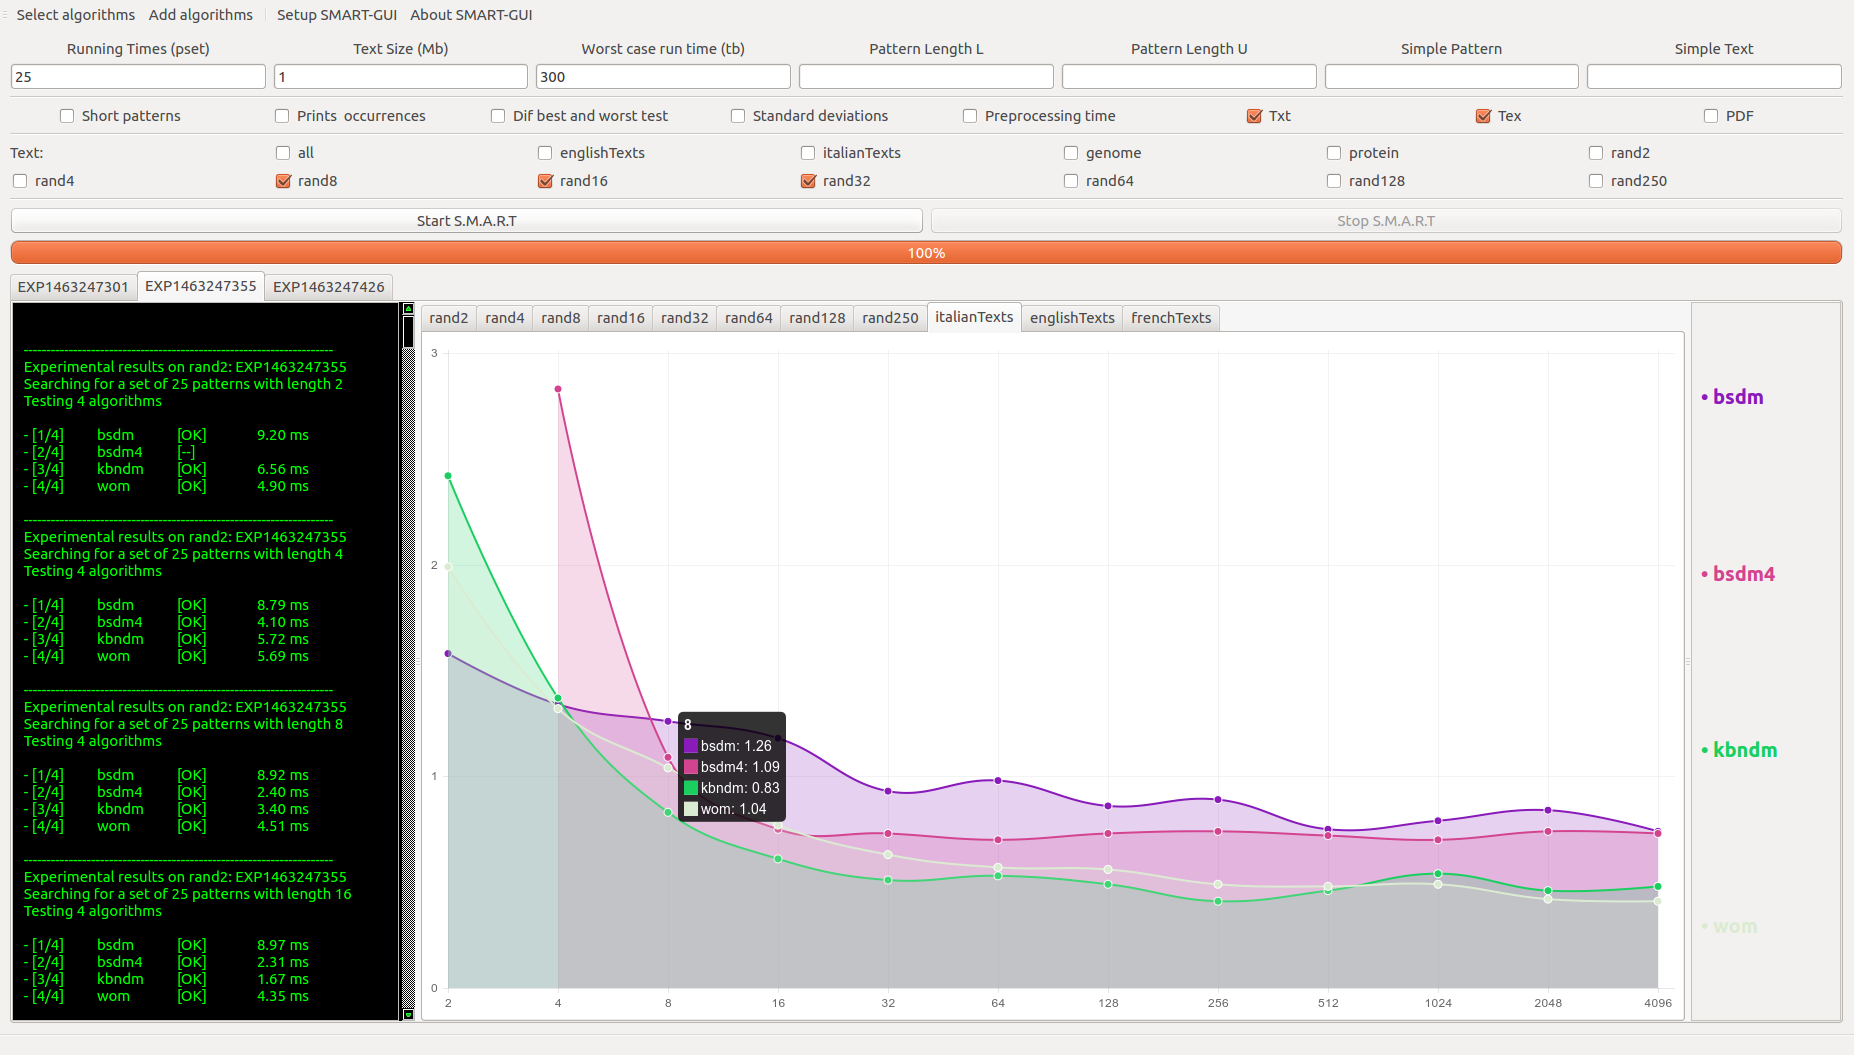
\includegraphics[width=5.5in]{Figure/smartGUI.png}}
    \caption{Anteprima di SMART-GUI.}
    \label{fig:esempio}
\end{figure}

La schermata centrale propone i grafici prodotti dal tool a serguito di un processo computativo. Il lato sinistro, invece, simula le fasi computative proprio come la controparte da terminale del tool. Ulteriori campi di input permettono di specificare i parametri più variegati.

\vspace{3mm}

Tuttavia, l'autore di questa tesi ha individuato empiricamente alcuni problemi di compatibilità relativi alle librerie impiegate per renderizzare l'interfaccia grafica, fra cui \verb|QtLibrary| e \verb|libqtwebkit4|. Potrebbe essere estremamente difficoltoso, o comunque lento e poco efficiente, installare questa versione SMART dotata di interfaccia grafica, per l'utente medio. Numerosi problemi relativi a versioni non più supportate o obsolete delle dipendenze in uso rendono, dunque, la versione da terminale di SMART quella più mantenibile, robusta e funzionante, che risulta altresì immediata e semplice da installare ed utilizzare.

\section{Conclusioni e criticità del software}

Inizialmente, il tool SMART è stato analizzato e studiato come possibile candidato ad ospitare algoritmi come \verb|scMAW|. In generale, si parla di algoritmi che sfruttano le minimal absent words e la metrica LW per indicare la similitudine fra le stringhe oggetto di confronto. Dopo un'attenta analisi e a seguito delle dovute considerazioni, risulta che SMART non sia adeguato né per \verb|scMAW|, né per tutti gli algoritmi che, analogamente a quest'ultimo, 

E' banale osservare come \verb|scMAW| e SMART, in relazione a quanto analizzato in questo Capitolo e nei Capitolo 2 e 3, non possa essere integrabile nel tool secondo i metodi previsti dagli autori. Difatto, come delineato nel Capitolo 4.2, gli algoritmi in via di integrazione devono seguire schemi ben precisi e non posso, almeno nella forma dei parametri accolti e dei tipi restituiti, divergere dalle condizioni vincolanti della piattaforma. Nello specifico, SMART impone la restituzione del numero di occorrenze di un certo pattern in un determinato corpo di testo. Invece, \verb|scMAW| prevede la generazione di un risultato di più ampio respiro, quale un file FASTA.OUT (descritto nel Capitolo 5), contenente indici LW per insiemi ben definiti di stringhe.

Risulta fondamentale osservare come SMART agisca in funzione del numero di occorrenze dei pattern risoluti, mentre gli algoritmi in esame - proprio perché sfruttano l'informazione negativa (nella forma di \textit{absent words} e  simili) piuttosto che quella positiva - sono esclusivamente in grado di fornire un grado di similitudine fra gli elementi input, restringendoli fra l'altro ad un alfabeto specifico, quale quello del genoma. 

Risulta evidente che SMART non sia stato pensato per accogliere algoritmi di questa tipologia. L'implementazione di \verb|scMAW| non può essere adeguata alla forma richiesta dal tool, né sarebbe opportuno tentare di convertire output così distanti e sconnessi fra loro per tentare di assecondare i vincoli del software. 

\vspace{3mm}

Per questi motivi, oltre che per motivi di natura didattica, è stato deciso di realizzare un software ad hoc per integrare algoritmi come quello in esame. 

\vspace{3mm}

In particolare, il tool in sviluppo dovrà essere in grado di elaborare algoritmi che restituiscono un file FASTA.OUT, prendendone in input uno di tipo FASTA e ammettendo esclusivamente l'alfabeto del genoma. Il tool dovrà, similmente a SMART, elaborare dei grafici illustrativi per permettere non solo considerazioni di tipo comparativo sulla qualità degli algoritmi selezionati, ma anche sulla loro correttezza e robustezza in termini degli indici LW restituiti a seguito dell'elaborazione.

\chapter{Realizzazione del tool LW Index}
    In virtù delle mancanze del tool SMART delineate nel Capitolo 5, si è deciso di procedere alla realizzazione di un'applicativo web ad hoc per sopperire alle lacune del suddetto tool.

\vspace{3mm}

Il tool in sviluppo, denominato LW Index, in riferimento all'omonima metrica presentata nel Capitolo 2, è definito come SMART-like, o simil-SMART. Il tool SMART permetteva di confrontare una serie di algoritmi di confronto fra stringhe, a prescindere dalla loro natura, e generare conseguentemente dei grafici predisposti a valutazioni di natura qualitativa da parte dell'utente.

Benché sia disponibile in una versione parallela adoperante un'interfaccia grafica, SMART nasce come programma da terminale; nella fattispecie, come si è osservati nel Capitolo 4, è in grado di produrre - a partire da una collezione di stringhe (o più banalmente un testo) e uno spettro di algoritmi selezionati - una pagina web costruita tramite elementi di HTML, CSS e JavaScript. 

D'altro canto, l'interazione dell'utente nasce e muore nel contesto del terminale: difatto, la pagina web autogenerata da SMART è di mera consultazione e non prevede ulteriore interazione con l'utente.

\vspace{3mm}

L'obiettivo è dunque di creare un tool che riesca ad accogliere algoritmi basati sulla metrica LW, incompatibili coi metodi di elaborazione e computazione di SMART; si noti, in ogni caso, che la metrica LW e le \textit{minimal absent words} sono strettamente legate, motivo per cui il tool è stato pensato specificamente per algoritmi che, oltre a misurare la similitudine con la metrica LW, facciano uso di \textit{minimal absent words} e derivati nella loro composizione funzionale.

\section{Progettazione del tool}

    Si osservi che, d'ora in poi, l'espressione "tool in sviluppo" sarà utilizzata in maniera intercambiabile col suo proprio nome, quale LW Index. 

    \subsection{Caratteristiche e funzionalità ad alto livello}

        In generale, il tool in sviluppo permetterà di creare grafici (al più 4) in maniera del tutto simile al tool SMART; svuotare la tavola di lavoro (cioè distruggere i grafici--tutti o individualmente) e analizzare i grafici. Creare un grafico significa, ad alto livello, generare un'istanza di lavoro vuota, popolabile con dati e stringhe durante la fase di analisi. 
        
        Analizzare i grafici significa porre in evidenza uno dei grafici fra quelli creati sulla tavola di lavoro ed effettuare una serie di azioni, fra cui visionare, in maniera grafica o testuale, il processo computazionale svolto per arrivare a quei dati, e modificare i grafici aggiungendo, rimuovendo o alterando stringhe. 
        
        \vspace{3mm}
        
        E' importante sottolineare che modificare il grafico significa necessariamente creare una nuova richiesta computativa.
        
        \vspace{3mm}
        
        Sarà possibile cambiare algoritmo. Il tool sarà sufficientemente versatile da accogliere un insieme diversificato di algoritmi che hanno in comune l'impiego della stessa metrica di similitudine fra stringhe, quale l'indice LW.
 
        \vspace{3mm}
 
        I grafici rappresenteranno sulle ascisse le stringhe (su alfabeti ben definiti) e sulle ordinate il corrispettivo indice LW. Questo significa che, per ogni stringa, il grafico produrrà una curva distinta a cui assocerà un indice LW per ogni altra stringa di quel grafico.  
        
        Come accennato, il tool potrà ospitare al più 4 grafici per volta, ed ogni grafico sarà analizzabile e modificabile indipendentemente dagli altri.

    \subsection{Architettura dell'applicazione}
    
        Il tool LW Index adotterà un'architettura web di tipo client-server. L'utente si interfaccerà con l'applicazione attraverso un browser web come Google Chrome o Mozilla Firefox. Questa scelta risulta funzionale perché il tool dovrà offrire un maggior numero di opzioni d'interazione rispetto a SMART, e preservare i dati fra un'esecuzione e l'altra.
        
        \vspace{3mm}
        
        Gli algoritmi di confronto dovranno essere ospitati sul server in una specifica directory. 
        
        \vspace{3mm}
        
        Nel dettaglio, l'utente potrà avviare l'applicativo tramite terminale. Una volta lanciato uno specifico comando, un'istanza del client (ossia una pagina web) si aprirà e contemporaneamente il webserver si avvierà.
        
        \vspace{3mm}
        
        Fra le caratteristiche proposte al punto 5.1.1, l'unica funzionalità che richiede l'intervento del server è la modifica di un grafico. Si noti che, pure se un grafico è vuoto (e cioè non è stato ancora popolato da stringhe), si sta affrontando un'operazione strettamente di modifica. Ogni volta che si richiede di aggiungere, eliminare o modificare stringhe, e si avvia il processo computativo alla pressione di un tasto, il webserver dovrà essere contattato e informato sulla natura della richiesta, per poi trattare i dati in put ed eventualmente fornire in output i dati necessari alla generazione del grafico.
    
    \subsection{Scelta delle tecnologie impiegate nell'implementazione}
    
        L'applicativo sarà implementato con tecnologie moderne e convenienti, al fine di semplificare la fase di implementazione e ridurre al minimo i casi di errore da gestire. Si è dunque deciso di implementare il webserver e il backend dell'applicazione con Node, mentre il frontend del client con React. Il techstack costituito da React e Node è un'alternativa popolare all'utilizzo grezzo della tecnologia fondamentale dalla quale entrambi derivano, quale JavaScript.  
        
        \vspace{3mm}
        
        Per ciò che concerne il frontend, le applicazioni web implementate in React possono sfruttare JavaScript o TypeScript; quest'ultimo, notoriamente, è un'alternativa al primo ed è caratterizzato da una forte tipizzazione, del tutto mancante invece in JavaScript. 
        
        E' stato deciso di implementare il tool in sviluppo con la variante TypeScript di React.
        
        \vspace{3mm}
        
        Per ciò che concerne il backend, Express, popolare framework di Node, è stato selezionato per l'implementazione del webserver. Express permette di avere immediatamente disponibile un ambiente di sviluppo facilmente configurabile, al quale è possibile agganciare nuove API attraverso sistemi di routing personalizzabili. 
        
        Questa scelta risulta immediata poiché il server dovrà ammettere un singolo processo elaborativo, quale la trasmissione dei dati fra il client e l'eseguibile dell'algoritmo selezionato per la computazione, sintetizzabile in un'unica route del webserver. 
        
        \vspace{3mm}
        
        Ulteriori informazioni su React e Node sono reperibili in italiano rispettivamente ai seguenti indirizzi: \url{https://it.reactjs.org/} e \url{https://nodejs.org/it/}.
    
    \subsection{Struttura del filesystem dell'applicazione}
    
        A basso livello, la struttura del filesystem di LW Index si presenta come segue. La directory \verb|/api| conterrà il sorgente del backend, mentre la directory \verb|/client| il sorgente del frontend. Entrambe le directory sono contenute in un macrospazio di lavoro denominato \verb|codebase|.
    
        \begin{verbatim} 
            ~/{root}         
                /api
                /client
        \end{verbatim}
        
        Il contenuto predefinito di ambo le cartelle è costituito dai file predefiniti di React (variante TypeScript) e Node (variante Express). Una volta installati rispettivamente React e Node, infatti, le due cartelle si popoleranno con un insieme di file critici per il funzionamento dell'applicazione. Dalla struttura base fornita dal processo di installazione, è possibile iniziare ad implementare le funzionalità dell'applicativo.
        
        \vspace{3mm}
        
        Gli algoritmi di confronto saranno collezionati in una sub-directory di \verb|/api| che prenderà il nome di \verb|/algo|. La cartella \verb|/algo| presenterà, dunque, un insieme di sottocartelle, ognuna contenente il codice sorgente del proprio algoritmo.
        
       \begin{verbatim} 
            /api         
                /algo
                    /Algoritmo_1
                    /Algoritmo_2
                    ...
                    /Algoritmo_N
        \end{verbatim}
        
        Il contenuto della i-esima cartella \verb|/Algoritmo_i| è del tutto indipendente rispetto al resto dell'applicativo. Questo significa che gli algoritmi possono essere strutturati in qualsiasi modo (ad esempio utilizzare certe strutture dati piuttosto che altre), a patto che siano implementati in C o C++ e che risultino pre-compilati ed eseguibili una volta inseriti nella propria directory. Non è, inoltre, possibile avere casi di omonimia fra directory ospitanti i sorgenti degli algoritmi.
        
\section{Implementazione del tool}

\subsection{Backend e Webserver}
    
La macrocartella \verb|/api|, come accennato nel paragrafo 5.1.2 e 5.1.4, conterrà l'implementazione del backend dell'applicativo, incluse le routine logiche necessarie al webserver per accogliere, processare e modellare le richieste in arrivo dal webclient in modo corretto.
    
Una volta installato Express seguendo le istruzioni presente sul sito del framework, un vasto numero di file si autogenererà nella cartella in cui si è lanciato il comando d'installazione. Di questi file, sarà sufficiente modificare esclusivamente \verb|app.js| e \verb|routes/computeAPI.js|. Si noti che quest'ultimo file dev'essere creato manualmente. 

\subsubsection{Backbone: App.js}

Il file \verb|app.js| avrà la seguente struttura:

\begin{itemize}
  \item In cima, una serie di require() per imporre l'utilizzo di specifiche dipendenze di routing, parsing e pathing, oltre che di gestione di errori.
  \item Immediatamente dopo il listing delle dipendenze, comandare l'utilizzo di Express tramite \verb|app = express()|
  \item Successivamente, indicare le routes (punti di contatto delle API) da rendere disponibili all'esterno, e in particolare al webclient, tramite \verb|app.use('/api/computeAPI')|. 
  \item Infine, stabilire le modalità di gestione degli errori HTTP più comuni, come il 404.
  \item Come ultimo passaggio, esportare il nucleo del backend come modulo tramite \verb|module.exports = app|.
\end{itemize}
    
\begin{sexylisting}{app.js}
var createError = require('http-errors');
var express = require('express');
var path = require('path');
var cors = require('cors');
var bodyParser = require('body-parser');

[..]

var computeRouter = require('./routes/computeAPI');

var app = express();

[..]

app.use('/api/computeAPI', computeRouter);
app.use(function (req, res, next) {
	next(createError(404));
});

[..]

module.exports = app;
\end{sexylisting}

Per quanto sia possibile arricchire ulteriormente \verb|app.js|, non risulta necessario nel nostro caso. Infatti, questo file - che rappresenta il backbone, o spina dorsale, del backend - ha semplicemente due funzioni:

\begin{itemize}
    \item Segnalare casi di errore, ed eventualmente ridirezionare la richiesta
    \item Accogliere la richiesta di computazione del confronto, di conseguenza accedere ed invocare la route \verb|/api/computeAPI|. Quando il client spedirà una richiesta verso \verb|/computeAPI|, il server sarà in grado di applicare un'interfaccia logica fra l'API \verb|/computeAPI| e il contenuto del file \verb|routes/computeAPI.js|. In effetti, il contenuto di quest'ultimo file è il cuore del backend, e ha il compito di gestire le richieste in entrare e restituire dei dati come risposta.
\end{itemize}

\subsubsection{Router: ComputeAPI.js}

Il webclient, al momento della spedizione di una nuova richiesta computativa, dovrà inserire come endpoint della richiesta la route \verb|/computeAPI|, indicando l'indirizzo di rete del webserver come origine. L'unica richiesta che questa route è in grado di accogliere è di tipo \textit{POST}. 

Inoltre, la route ammette esclusivamente richieste sicure, che rispettino il protocollo CORS e che prevedano JSON come formato comune di elaborazione.

\begin{sexylisting}{computeAPI.js > Header}
router.post('/', function (req, res, next) \{
	res.set({
		'Content-Type': 'application/json',
		'Access-Control-Allow-Origin': '*',
	});
	
    [..]
\}
\end{sexylisting}

A basso livello, l'obiettivo del webserver è generare un file FASTA a partire da un insieme di stringhe in input; successivamente, il webserver dovrà fornire il file FASTA appena creato in pasto all'algoritmo selezionato. A questo punto, il webserver dovrà attendere l'esecuzione dell'algoritmo e, in particolare, che quest'ultimo stampi i risultati sul file di output. Infine, il webserver dovrà interpretare il file di output e convertirne i dani estrapolati come JSON. A questo punto, il webserver sarà in grado di rispondere al webclient con i dati necessari per generare il grafico.

\vspace{3mm}

Il primo step risulta, dunque, convertire il JSON pervenuto dal webclient in formato FASTA. Il fulcro del lavoro di conversione giace nell'interpretare le stringhe contenute nel corpo della richiesta ed inserirle con le opportune tabulazioni e spaziature in un file di testo vergine; similmente, ogni stringa dovrà essere associata ad un indice incrementale con la quale potrà essere, in seguito, identificata visivamente sul grafico prodotto.

\begin{sexylisting}{computeAPI.js > Conversione del JSON in FASTA}
const strings = req.body.strings;
	
strings.forEach((string) => {
	FASTA += '>' + index + '\n';
	FASTA += string.toUpperCase() + '\n';
	stringNames.push(string.toUpperCase());
	++index;
});
\end{sexylisting}

Di seguito si propone il template di un file FASTA e esempio popolato da quattro stringhe.

\begin{sexylisting}{computeAPI.js > Template di un file FASTA}
>[index]
STRING
>[index 2]
STRING 2
...
>[index N]
STRING N
\end{sexylisting}

\begin{sexylisting}{computeAPI.js > Esempio di un file FASTA}
>1
GGTAAC
>2
AAAAAACCCTGTGT
>3
TTTTATATACC
>4
CCGTTTAAACC
\end{sexylisting}

Risulta altresì fondamentale elaborare un protocollo di denominazione che generi nomenclature univoche sia per i file di input, che per i file di output. Si decide di utilizzare il timestamp tramite \verb|Date.now()| per creare associazioni uno-a-uno fra i due file. E' importante osservare che i file saranno gestiti in UTF-8.

\vspace{5mm}

I file di input saranno costruiti come segue.

\begin{table}[H]
\begin{tabular}{@{}ll@{}}
\toprule
\textbf{Costante}                    & \textbf{Contenuto}               \\ \midrule
\textit{\textbf{\_\_IN\_FILE\_NAME}} & algo + '-request-' + Date.now()  \\
\textit{\textbf{\_\_IN\_EXTENSION}}  & '.fasta';                        \\
\textit{\textbf{\_\_IN\_DIRECTORY}}  & './algo/' + algo + '/lw-index/'; \\ \bottomrule
\end{tabular}
\end{table}

Analogamente, i file di output saranno costruiti come segue.

\begin{table}[H]
\begin{tabular}{ll}
\hline
\textbf{Costante}                     & \textbf{Contenuto}                      \\ \hline
\textit{\textbf{\_\_OUT\_FILE\_NAME}} & Date.now();                             \\
\textit{\textbf{\_\_OUT\_EXTENSION}}  & '.fasta.out';                           \\
\textit{\textbf{\_\_OUT\_DIRECTORY}}  & './algo/' + algo + '/lw-index/result/'; \\ \hline
\end{tabular}
\end{table}

Poiché gli algoritmi sono lanciati da eseguibili ottenuti come risultato di bundle precompilati generalmente adatti ad un ambiente Linux, e riservandoci l'abilità di poter sfruttare il tool in sviluppo anche su ambiente Windows, si decide di utilizzare Windows Subsystem for Linux (WSL) per lanciare gli eseguibili degli algoritmi. E' sufficiente \textit{spawnare} (ossia istanziare) un terminale WSL e utilizzare STDIN, STDOUT e STDERR come un qualsiasi ambiente dotato di stream di input e output.

In questo modo, è possibile lanciare l'eseguibile dell'algoritmo selezionato simulando l'immissione di un comando personalizzato. Immediatamente dopo, per motivi di integrità dell'input, chiudiamo il flusso STDIN tramite \verb|end()|.

\begin{sexylisting}{computeAPI.js > Avvio dell'esecuzione dell'algoritmo}
wsl.stdin.write(
	'./algo/scMAW/sc-maw -a DNA -i ' +
	__IN_FILE +
	' -o ' +
	__OUT_FILE +
	'[opzioni]'
);

wsl.stdin.end();
\end{sexylisting}

Si osservi che, nelle fasi di integrazione di nuovi algoritmi, basterà sostituire \verb|scMAW|, l'unico algoritmo integrato in maniera predefinita nel tool, con una variabile di tipo stringa.

\vspace{3mm}

A questo punto, l'algoritmo eseguirà in autonomia i propri sottoprocessi. Il webserver rimarrà in attesa di un riscontro sullo standard output STDOUT. La chiusura del processo di WSL fungerà da indicatore al router di iniziare ad estrapolare ed interpretare i dati dal file di output.

\vspace{3mm}

Il file di output sarà di tipo FASTA.OUT ed è strutturato come segue.

\begin{sexylisting}{computeAPI.js > Template di un file FASTA.OUT}
[# Numero di stringhe]
[index 1]	 Lw(1, 1)   LW(1, 2)    LW(1, n)
[index 2]	 LW(2, 1)   LW(2, 2)    LW(2, n)
...	
[index N]	LW(n, 1)    LW(n, 2)    LW(n, n)
\end{sexylisting}

\begin{sexylisting}{computeAPI.js > Esempio di un file FASTA.OUT}
3
1	0.000000	0.861111	2.751123	
2	0.861111	0.000000	1.989003	
3	2.751123	1.989003	0.000000
\end{sexylisting}

La struttura prevede una riga per ogni stringa in input. Ogni stringa sarà dotata di una colonna per ogni stringa in input, più uno. La prima colonna di ogni riga rappresenta l'indice della stringa (da 1 a $N$), mentre la prima riga del file contiene il numero di stringhe.

Tralascinado la prima colonna, le colonne rimanenti di ogni riga eccetto la prima conterranno il valore della matrica LW fra la stringa rappresentata dall'indice di quella riga, e ogni altra stringa nell'insieme in input. Questa struttura permette di avere una visione complessiva delle similitudini fra tutte le stringhe in esame.

\vspace{3mm}

$LW(i, j)$ restituirà la similitudine (in float) fra la stringhe $i$ e la stringa $j$. Banalmente, $LW(i, i) = 0$.

\vspace{3mm}

E' possibile consultare il Capitolo 2 per ulteriori informazioni circa il calcolo grezzo dell'indice LW.

\vspace{3mm}

Il file risulta di semplice lettura. Infatti, è sufficiente troncare le singole righe, e successivamente gli spazi tabellari, per individuare la matrice di indici LW desiderata. Questa matrice rappresenta il risultato atteso dall'algoritmo, e sarà incapsulato nella proprietà \verb|graphData: result| di \verb|responseData|. Allo stesso tempo, l'algoritmo terrà conto del tempo impiegato (in millisecondi) per eseguire l'algoritmo in funzione delle stringhe in input, e depositerà questo dato nella proprietù \verb|quality.time|, rendendo disponibile future considerazioni qualitative da parte dell'utente.

\begin{sexylisting}{computeAPI.js > Conversione FASTA.OUT in JSON}
fs.readFile(__OUT_FILE, ENCODING, (err, data) => {
	if (err) throw err;
	var result = [], j = 0;

	const rows = data.split(/\r?\n/);
	rows.forEach((row) => {
		const splitData = row.split('\t');
		let string = stringNames[j++]
		let lw = [];

		splitData.shift();
		splitData.pop();
		splitData.forEach(
		    (data) => lw.push(data)
		);

		result.push({
			string: string,
			lw: lw,
		});
	});

	const responseData = {
		quality: {
			time: time,
		},
		graphData: result,
	};

	res.json(responseData);
});
\end{sexylisting}

\begin{figure}[ht!]
    \centering
    \tmpframe{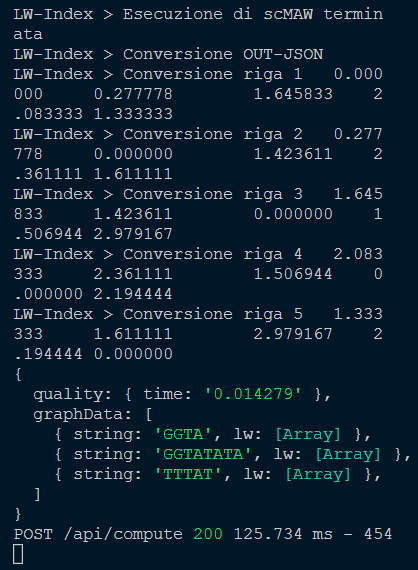
\includegraphics[width=4in]{Figure/console.png}}
    \caption{Anteprima di una porzione del processo di computazione svolto dal server}
    \label{fig:esempio}
\end{figure}


L'istruzione conclusiva \verb|res.json(responseData)| rappresenta la chiusura della richiesta e l'invio della risposta al client. A questo punto, il webserver rimarrà attivo e in attesa di nuove richieste da parte del client. Non eseguirà, in ogni caso, altre azioni in autonomia.

\subsection{Webclient e Frontend}

L'implementazione del frontend di una piattaforma web in React è dissimile rispetto ai metodi tradizioni di costruzione di siti web interattivi con tecnologie primitive come JavaScript. React, per definizione, è un framework per JavaScript che adotta una filosofia a componenti. Ogni elemento sulla pagina viene interpretato logicamente come un componente funzionale della piattaforma, dipendente o meno rispetto ad un componente padre, e contenente o meno uno o più componenti figli. 

I componenti React sono estremamente versatili e poliedrici, in grado di assumere connotazioni particolarizzanti in funzione degli obiettivi dello sviluppatore. 

Oltre a React, la marcatura della piattaforma sarà costruita tramite HTML e CSS. 

Per quanto si vorrebbe dare una spiegazione ampia e dettagliata di ogni singolo aspetto dell'implementazione del frontned, non è possibile data l'enorme mole di codice, che si attesta sull'ordine delle migliaia di righe al netto dei file autogenerati dal processo di installazione. Per questo motivo, il codice sorgente è liberamente e gratuitamente consultabile al seguente indirizzo: \url{https://github.com/v1enna/lw-index}.

\vspace{3mm}

Il sistema dovrà essere fornito di una dashboard interattiva e un menù laterale che permetta di effettuare operazioni. Le operazioni, essenzialmente, avranno il compito di alterare il contenuto della dashboard, e di conseguenza modificare lo stato dell'applicazione.
\newpage
\subsubsection{Dashboard e gestione dello stato}

Il menù laterale prevede tre macrosezioni: \textbf{Operazioni}, \textbf{Algoritmo} e \textbf{Debug}.

\begin{figure}[ht!]
    \centering
    \tmpframe{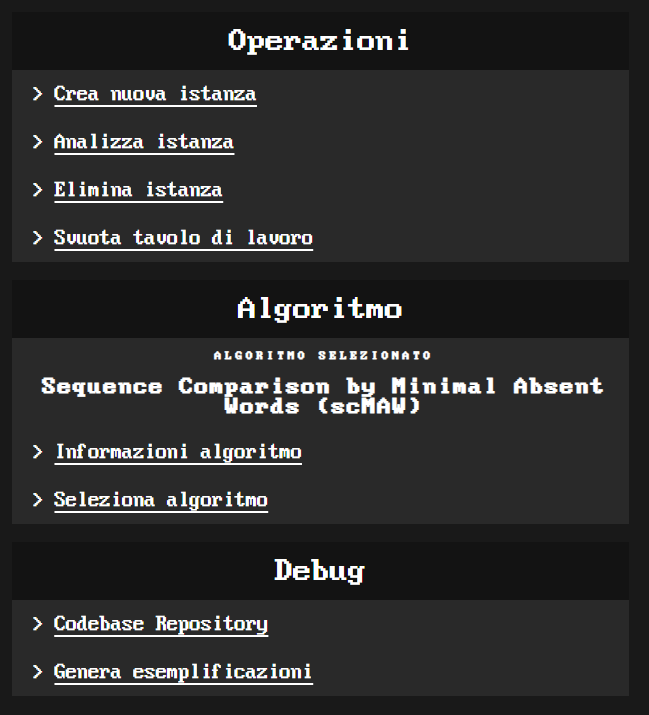
\includegraphics[width=5in]{Figure/menu.png}}
    \caption{Menù laterale della piattaforma. La pressione dei tasti produce alterazioni uniche in termini di contenuto dello spazio di lavoro (dashboard) e dello stato dell'applicativo.}
    \label{fig:esempio}
\end{figure}

\begin{itemize}
    \item La sezione \textbf{Operazioni} sarà l'area principale di interazione con l'utente. L'utente potrà creare nuove istanze di lavoro, analizzarle, eliminarle e svuota l'intera dashboard. Si osservi che 'tavolo di lavoro' e dashboard sono intercambiabili.
    \item La sezione \textbf{Algoritmo} fornisce informazioni critiche sull'algoritmo selezionato, permettendo inoltre di selezionarne di differenti. 
    \item La sezione \textbf{Debug} permette di generare una serie di grafici esemplificativi, riempiendo il tavolo di lavoro con quattro istanze popolate, e di accedere al codice sorgente dell'applicazione, che è open source.
\end{itemize}

\subsubsection{Fase di analisi delle istanze di lavoro}

E' possibile analizzare le istanze di lavoro a prescindere dal loro stato; di conseguenza, un'istanza è analisi anche se non ancora popolata da stringhe. Analizzare un'istanza trasformerà il tavolo di lavoro generale in un tavolo di lavoro specifico per l'istanza in analizi. Da questa schermata, è possibile effettuare la maggior parte delle operazioni previste dalle funzionalità ad alto livello indicate in precedenza.

\begin{figure}[ht!]
    \centering
    \tmpframe{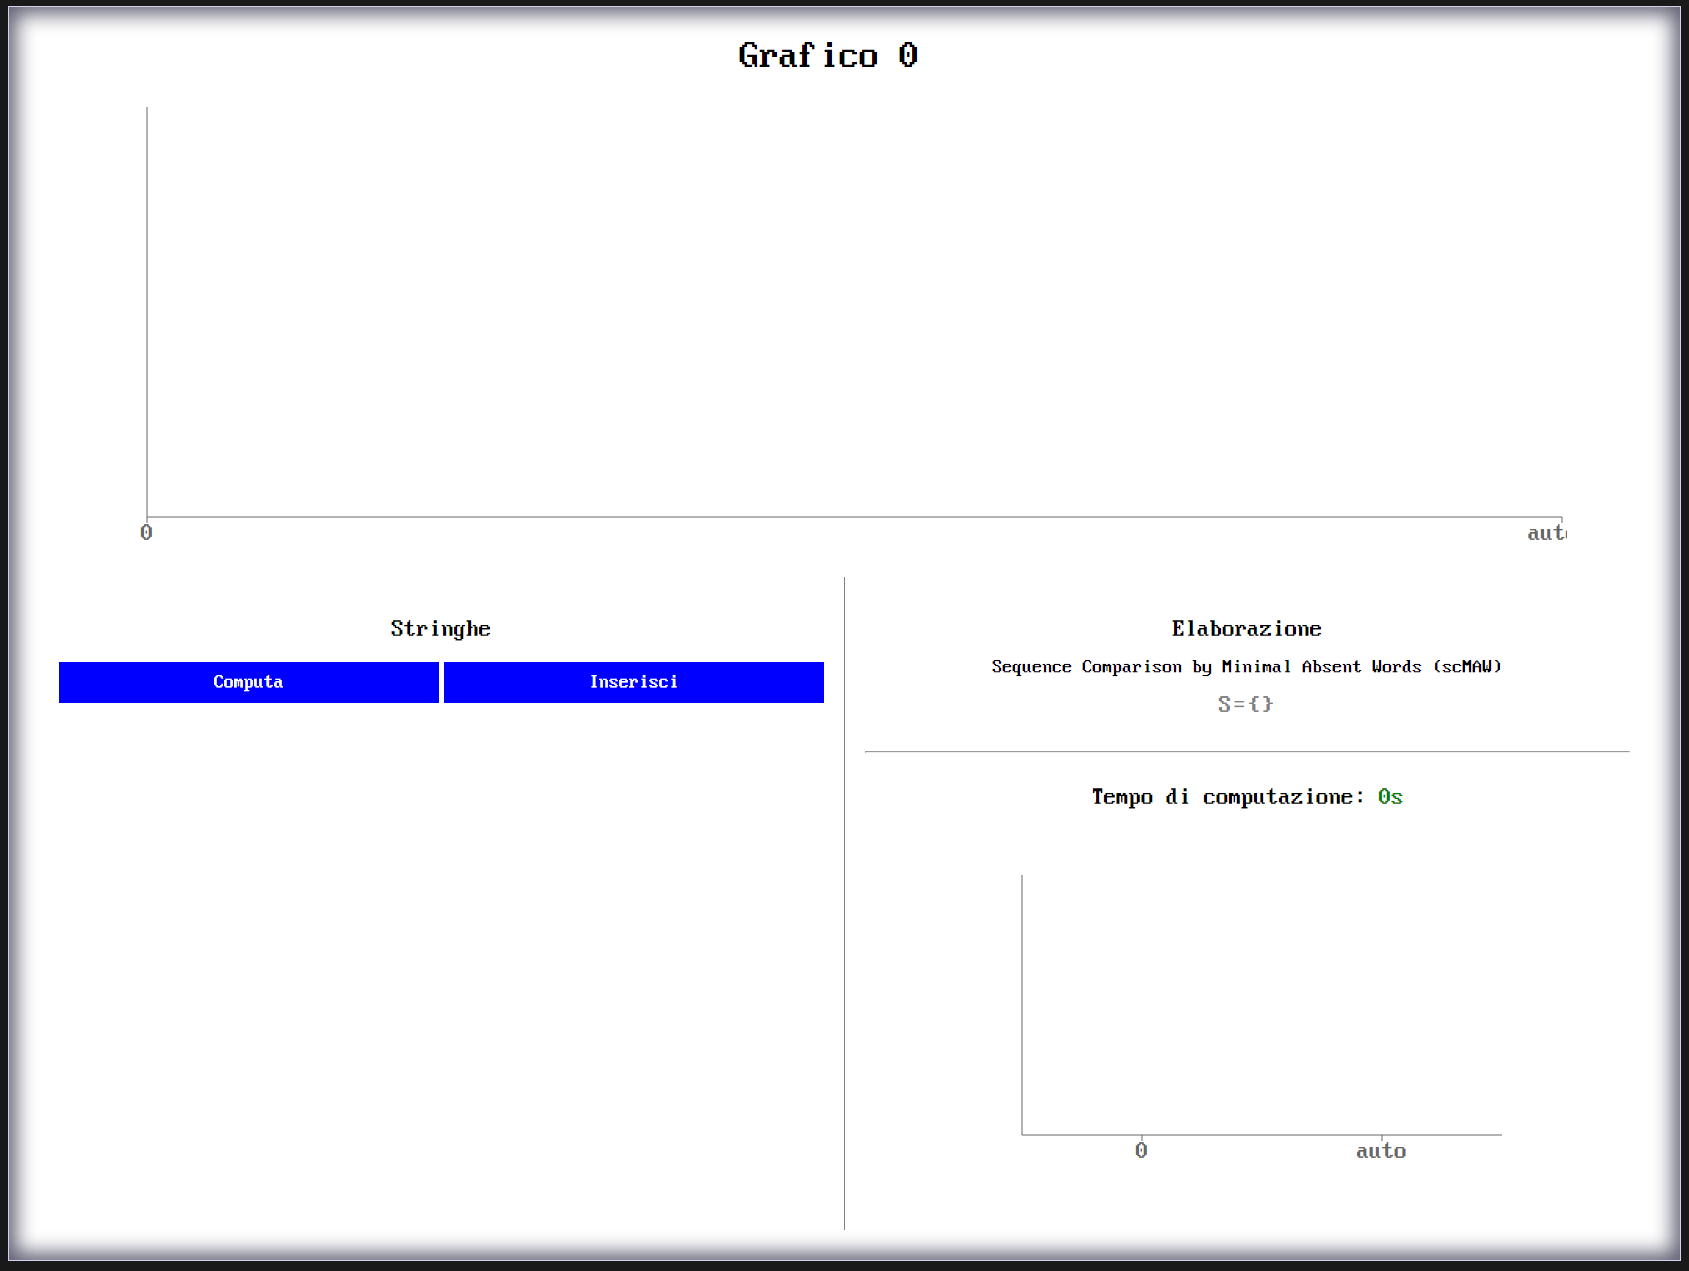
\includegraphics[width=6in]{Figure/analisi.png}}
    \caption{La fase di analisi prevede una schermata bianca divisa in due semispazi. Il semispazio superiore conterrà il grafico prodotto dalla computazione più recente (relativa all'istanza in analisi); il semispazio inferiore conterrà a sinistra i form di immissione delle stringhe, e a destra un grafico di comparazione qualitativa.}
    \label{fig:esempio}
\end{figure}

Se l'istanza in analisi è neonata o non popolata, il semispazio superiore della schermata sarà occupato da due assi esenti da curve. In alternativa, se l'istanza è stata precedentemente popolata o si richiede una nuova computazione in essere, il semispazio sarà occupato da un grafico ricco di tante curve quante le stringhe immesse nella parte sinistra del semispazio inferiore della schermata di analisi.

\begin{figure}[ht!]
    \centering
    \tmpframe{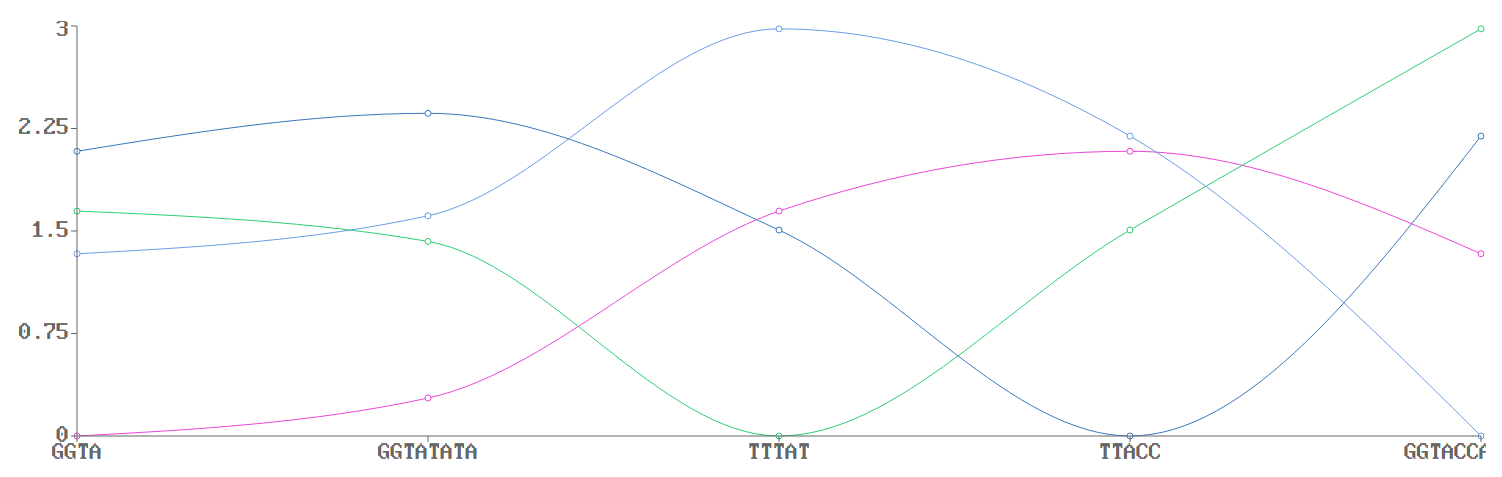
\includegraphics[width=6in]{Figure/grafico.png}}
    \caption{Esempio di grafico generato dal tool. I grafici rappresentano la similitudine fra le stringhe in input. Ciò significa che ogni curva rappresenta una stringa dell'insieme di stringhe fornito al momento della computazione. L'asse delle ordinate rappresenta gli indici LW, mentre quello delle ordinate rappresenta le stringhe.}
    \label{fig:esempio}
\end{figure}

La lettura del grafico è immediata, conoscendo la struttura di 

\subsubsection{Generazione automatica di grafici esemplificativi}

La voce \textit{Genera esemplificazioni} è particolarmente utile per avere un'anteprima del funzionamento dell'applicativo. Alla pressione, infatti, il tool autogenererà quattro grafici con dati casuali, simulando il processo di elaborazione di cui si occupa il server. Proprio perché i dati sono casuali, il riavvio dell'applicazione resetterà i parametri che generano i grafici, creandone di nuovi ogni volta. In figura un esempio visivo.

\begin{figure}[ht!]
    \centering
    \tmpframe{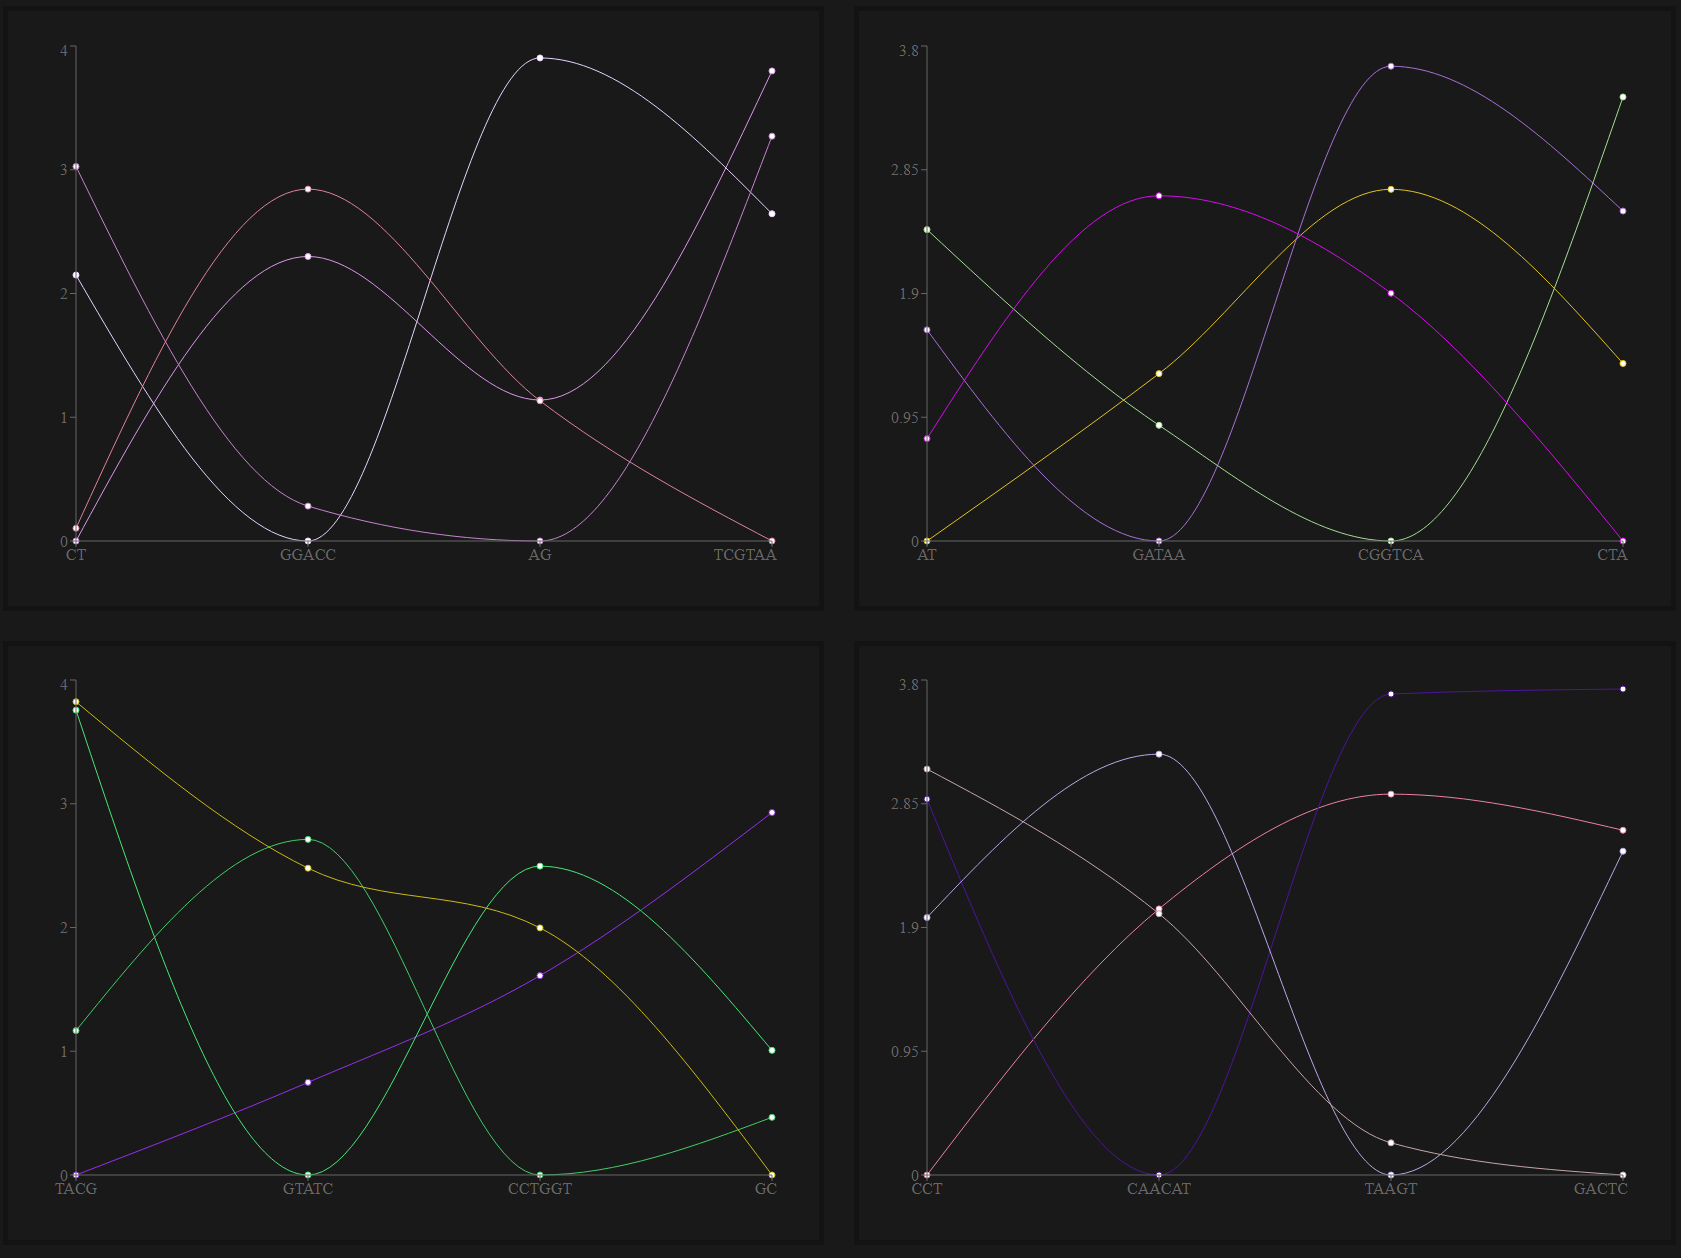
\includegraphics[width=6in]{Figure/esempi.png}}
    \caption{L'operazione di debug "Genera esemplificazioni" riempie il tavolo di lavoro con grafici casuali come in figura.}
    \label{fig:esempio}
\end{figure}

\begin{figure}[ht!]
    \centering
    \tmpframe{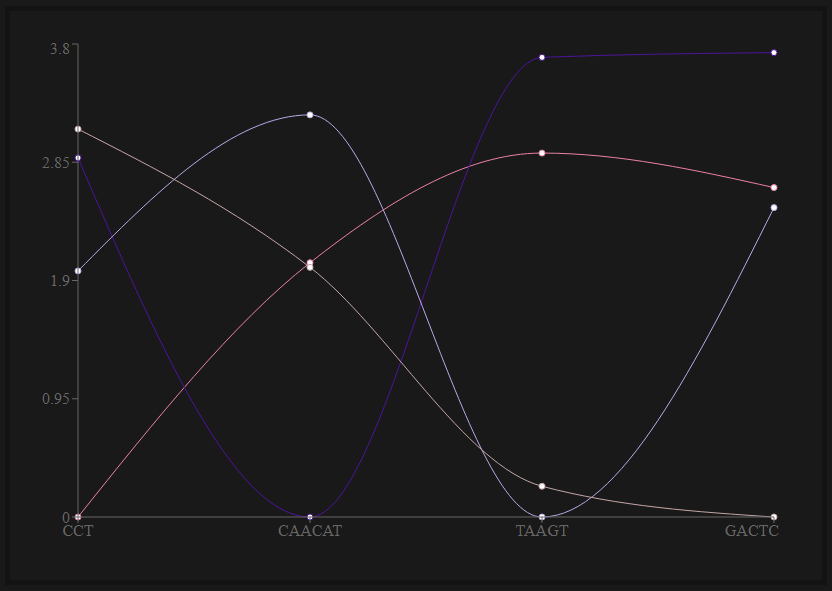
\includegraphics[width=6in]{Figure/singoloEsempio.png}}
    \caption{Dettaglio di un singolo grafico esemplificativo autogenerato tramite operazioni di debug.}
    \label{fig:esempio}
\end{figure}

\section{Esempi di utilizzo pratico}
    
\chapter{Conclusioni e possibili sviluppi futuri}
    Questo lavoro di tesi avevo lo scopo di esplorare, ad alto livello, le potenzialità dell'informazione negativa nell'ambito della bioinformatica, ed in particolare nella cornice del più ampio campo di lavori circa il confronto fra sequenze del genoma, benché sia applicabile - in generale - a stringhe su alfabeti ben definiti, come potrebbe essere quello proteico. 

Successivamente, il lavoro di tesi ha imposto lo studio approfondito di un algoritmo che facesse dell'informazione negativa, nella forma delle \textit{absent words} prima, e delle \textit{minimal absent words} poi, la nozione matematica critica nella sua composizione algoritmica. 

Lo studio ha dunque condotto al reverse engineering e alla comprensione generale del funzionamento del tool SMART che, dopo un'attenta revisione della natura dell'applicativo e delle modalità di elaborazione dei dati in input e ouput che adottasse, è risultato incompatibile con l'obiettivo generale di questo lavoro di tesi, il quale si prefissava - in origine - di integrare algoritmi come \verb|scMAW| in un tool di comparazione qualitativa.

\vspace{3mm}

Poiché SMART non è risultato adatto ai nostri fini, i lavori di tesi sono stati ridirenzionati, mutando in parte. Dato che non esisteva, al meglio delle conoscenze dell'autore di questa tesi,  e al momento della stesura di quest'ultima, un tool simil-SMART in grado di accogliere algoritmi che sfruttano l'informazione negativa e siano implementati nelle specifiche modalità indicate nei capitoli precedenti, si è deciso di realizzare un tool ad hoc, del tutto originale, adottante un'architettura client-server e implementato con tecnologie moderne e all'avanguardia. Si tratta di una one-page web-application che soddisfa a pieno i requisiti funzionali previsti dal progetto originario della tesi di laurea.

\vspace{3mm}

Risulta evidente che il tool oggetto di sviluppo sia ampiamente arricchibile con nuove funzionalità, e che sia sufficientemente versatile da accogliere un importante numero di algoritmi di confronto fra stringhe. Risulta altresì evidente che il tool possa essere notevolmente migliorato, soprattutto sul fronte dell'usabilità; d'altro canto, un possibile sviluppo futuro potrebbe essere rappresentato, similmente a SMART, dalla realizzazione di una controparte desktop, e dunque non basata su web-browser, dell'applicativo. Poiché il software tratta un ambito di così ampio respiro come quello dei confronti fra stringhe, è banale evidenziare come le modifiche apportabili all'implementazione - funzionale e non - siano innumerevoli (ad esempio, si potrebbe permettere all'utente di immettere direttamente file FASTA precompilati).

\vspace{3mm}

Il lavoro di tesi ha, in conclusione, evidenziato le potenzialità dell'informazione negativa nel quadro della bioinformatica, e come la questione del calcolo della similitudine fra stringhe sia, ad oggi, un argomento ancora ricco di spunti di riflessione e innovazioni scientifiche.

\printbibliography

\end{document}
